% Template for a Computer Science Tripos Part II project dissertation
\documentclass[12pt,a4paper,twoside,openright]{report}
\usepackage[pdfborder={0 0 0}]{hyperref}    % turns references into hyperlinks
\usepackage[margin=25mm]{geometry}  % adjusts page layout
\usepackage{graphicx}  % allows inclusion of PDF, PNG and JPG images
\usepackage{pmboxdraw}
\usepackage{verbatim}
\usepackage{docmute}   % only needed to allow inclusion of proposal.tex
\usepackage{parskip}
\usepackage{pdfpages}
\usepackage{listings}
\usepackage{amsmath}
\usepackage{amsfonts}

\usepackage{algorithm}
\usepackage{algpseudocode}
\usepackage[linguistics]{forest}
\usepackage[nocenter]{qtree}

\usepackage{todonotes} % remove


\lstset{basicstyle=\ttfamily, breaklines=true, columns=fullflexible}

\graphicspath{ {./images/} }

\newcommand{\quickwordcount}[1]{%
  \immediate\write18{texcount -1 -sum -merge -q #1.tex output.bbl > #1-words.sum }%
  \input{#1-words.sum} words%
}

\raggedbottom                           % try to avoid widows and orphans
\sloppy
\clubpenalty1000%
\widowpenalty1000%

\renewcommand{\baselinestretch}{1.1}    % adjust line spacing to make
                                        % more readable

\begin{document}

\bibliographystyle{plain}


%%%%%%%%%%%%%%%%%%%%%%%%%%%%%%%%%%%%%%%%%%%%%%%%%%%%%%%%%%%%%%%%%%%%%%%%
% Title

\pagestyle{empty}

\rightline{\LARGE \textbf{Jiaxin Wang}}

\vspace*{60mm}
\begin{center}
\Huge
\textbf{A Recursive Recurrent Neural Network Decoder for Grammatical Error Correction} \\[5mm]
Computer Science Tripos -- Part II \\[5mm]
Emmanuel College \\[5mm]
\today  % today's date
\end{center}
\thispagestyle{empty}

%%%%%%%%%%%%%%%%%%%%%%%%%%%%%%%%%%%%%%%%%%%%%%%%%%%%%%%%%%%%%%%%%%%%%%%%%%%%%%
% Proforma, table of contents and list of figures
\pagestyle{plain}
\pagenumbering{roman}
\newpage

\section*{Declaration}

I, Jiaxin Wang of Emmanuel College, being a candidate for Part II of the Computer
Science Tripos, hereby declare that this dissertation and the work described in 
it are my own work, unaided except as may be specified below, and that the dissertation
does not contain material that has already been used to any substantial
extent for a comparable purpose.

\bigskip
\leftline{Signed [signature]}

\medskip
\leftline{Date [date]}

\chapter*{Proforma}

{\large
\begin{tabular}{ll}
Candidate Number:   & -                       \\
Project Title:      & A Recursive Recurrent Neural Network \\
 & Decoder for Grammatical Error Correction \\
Examination:        & Computer Science Tripos -- Part II, 2022  \\
Word Count:         & \quickwordcount{diss}\footnotemark[1] \\
Code line count:    & 1182 \footnotemark[2]\\
Project Originator: & The Author \\
Supervisor:         & Dr Zheng Yuan, Dr Christopher Bryant
\end{tabular}
}
\footnotetext[1]{This word count was computed by 
\texttt{\textbackslash immediate\textbackslash write18\{texcount -1 -sum -merge -q diss.tex output.bbl > diss-words.sum\} and \textbackslash input\{diss-words.sum\} words}}

\footnotetext[2]{Code line count was computed
by \texttt{find ./model ./helper\_scripts -name "*.py" -print | xargs wc -l}
}
\stepcounter{footnote}

\section*{Original Aims of the Project}
This project aims to build a statistical machine translation (SMT) system for grammatical error correction using a recursive recurrent neural network (R\textsuperscript{2}NN) model as the decoder. It involves constructing a translation confidence based phrase pair embedding (TCBPPE) using a feedforward neural network (FNN) and a recurrent neural network (RNN), implementing the R\textsuperscript{2}NN model and training the R\textsuperscript{2}NN SMT system. A baseline SMT system (Moses) was built and trained with the same data. The R\textsuperscript{2}NN SMT was evaluated against baseline SMT on the grammatical error correction task using the $F_{0.5}$ metric.

\section*{Work Completed}
All the core goals of the project have been achieved. Two SMT systems were built, namely Moses SMT and R\textsuperscript{2}NN SMT. For Moses SMT, a baseline phrase-based SMT system was constructed. For R\textsuperscript{2}NN SMT, the recursive recurrent neural network was implemented from scratch and the phrase pair embedding (TCBPPE) was obtained to be used with R\textsuperscript{2}NN. Both systems were trained and tested with the same data. Finally, a comparison was carried out on the evaluation results of the two SMT systems for the task of grammatical error correction.

\section*{Special Difficulties}
None.

\section*{Acknowledgements}


\tableofcontents

\listoffigures

% \listoftodos

%%%%%%%%%%%%%%%%%%%%%%%%%%%%%%%%%%%%%%%%%%%%%%%%%%%%%%%%%%%%%%%%%%%%%%%
% now for the chapters
\pagestyle{headings}

\chapter{Introduction}
\pagenumbering{arabic}

\section{Motivation}

Grammatical Error Correction (GEC) is the task of producing a grammatically correct sentence given a potentially erroneous text while preserving its meaning. One of the many motivations behind this task is that it plays a significant role in helping learners of a foreign language understand the language better. Being an ESL (English as a second language) learner myself, it is often difficult for me to spot the errors in my English writing since English grammar is quite different from that of my first language. Native English speakers may wish to use a GEC system to avoid mistakes in their writing, especially in a professional environment (e.g. work emails). 

One common approach to GEC, SMT-based GEC, is to treat GEC as a translation problem and use a statistical machine translation (SMT) system to solve it. We train an SMT system that takes an erroneous source sentence as input and the grammatically correct sentence as the expected output. By searching for the best `translation' from the source sentence, the aim is to find a grammatically correct sentence that preserves the meaning of the original sentence.

Liu et al. proposed a novel model for SMT using a \textit{recursive recurrent neural network} (R\textsuperscript{2}NN)\cite{r2nn}. It has a tree structure similar to a recursive neural network, with recurrent input vectors to encode global information that cannot be generated by the child node representations. In the paper, they showed that their R\textsuperscript{2}NN SMT model achieved better performance than a state-of-the-art baseline system on a Chinese-to-English translation task. However, they did not publish their code, and no implementation of such an R\textsuperscript{2}NN SMT model is publicly available.

It is therefore of interest to implement such a neural network and apply it to the task of GEC. For one, publishing the code could benefit other researchers in this area who are interested in NLP (natural language processing), GEC, and neural networks. For another, if the R\textsuperscript{2}NN model is proven to be useful for GEC, it could help with developing better GEC systems and assist millions of English learners.

\section{Problem Overview}

An SMT system has four components: a language model (LM) which computes the probability of a given word sequence being valid, a translation model (TM) which constructs mappings of phrases between source and target corpora and calculates translation probabilities, a reordering model (RM) which handles phrase reordering, and a decoder which looks for the best translation candidate\cite{yuan2017phd}. The R\textsuperscript{2}NN model proposed by Liu et al. was used in the end-to-end decoding process of SMT, i.e. as a decoder. The goal of this project is to implement such a decoder, integrate it into an SMT system, apply it to GEC and evaluate its performance against a baseline SMT system. 

The GEC system should aim to correct all types of errors in non-native English text, including grammatical, lexical and orthographic errors, as defined in the BEA 2019 Shared Task\cite{bryant-etal-2019-bea}. Lexical errors are mistakes at the word level, such as wrong choice of words that do not fit in their context. Grammatical errors violate the grammar of a language, such as in subject-verb agreement. Orthographic errors include spelling errors but also casing errors (e.g. upper and lower case) and punctuation errors.

Moses\cite{moses} was used as the baseline SMT system to be evaluated against the R\textsuperscript{2}NN SMT. Moses is a toolkit commonly used for statistical machine translation. The toolkit contains a decoder (Moses decoder) and various tools for training and tuning. It also provides a user guide on how to use the decoder together with other models to build a SMT system. For this project, I built and trained a Moses SMT system. I also implemented and trained an R\textsuperscript{2}NN SMT system which uses the R\textsuperscript{2}NN model as the decoder. Finally, I compared the performance of both systems on the task of grammatical error correction.

\section{Related Work}

The paper\cite{r2nn} by Liu et al. discussed the structure of R\textsuperscript{2}NN and how it can be used as a decoder.  They also proposed a way to initialise the phrase pair embedding called \textit{translation confidence based phrase pair embedding} (TCBPPE) to generate the leaf nodes. After training the system on data from the IWSLT 2009 dialog task\cite{paul-2009-overview}, they tested the system on a Chinese-to-English translation task. Finally, they evaluated their system against a baseline decoder using the case insensitive IBM BLEU-4 method\cite{10.3115/1073083.1073135}. Details of R\textsuperscript{2}NN and TCBPPE are discussed in the following chapters.

SMT systems have been successfully used for the task of grammatical error correction. Yuan and Felice\cite{yuan-felice-2013-constrained} applied Moses SMT with GIZA++ and IRSTLM to grammatical error correction in the CoNLL-2013 Shared Task\cite{ng-etal-2013-conll}. Junczys-Dowmunt and Grundkiewicz\cite{junczys-dowmunt-grundkiewicz-2014-amu} developed a GEC system based on an SMT system, namely phrase-based Moses\cite{moses}, and they ranked third place in the CoNLL-2014 Shared Task\cite{ng-etal-2014-conll}. They also discussed the improvement that can be achieved by parameter tuning towards the evaluation metric for GEC in phrase-based SMT systems\cite{junczys-dowmunt-grundkiewicz-2016-phrase}. Yuan et al.\cite{yuan-etal-2016-candidate} discussed how SMT can be applied to GEC and how a re-ranking model can improve the performance of SMT-based GEC system. 

This project aims to implement the R\textsuperscript{2}NN together with TCBPPE in the paper\cite{r2nn} and build a SMT system. A phrase-based Moses SMT system\cite{moses} was built to be used as a baseline system. Both systems were applied to GEC and then evaluated by the ERRANT scorer\cite{bryant-etal-2017-automatic}\cite{felice-etal-2016-automatic}, the official evaluation tool of the BEA 2019 Shared Task\cite{bryant-etal-2019-bea}.


\chapter{Preparation}
\textit{This chapter describes the work done for preparation. Section \ref{section:start} gives an overview of my starting point. Section \ref{section:theory} discusses the background knowledge that helped me understand the nature of my project better. In section \ref{section:requirement} I present a list of requirements that should be fulfilled by my project. In the end, I explored the dataset and tools to be used in my project.}

\section{Starting Point}\label{section:start}

The goal of this project is to implement the R\textsuperscript{2}NN decoder proposed in the paper \textit{A Recursive Recurrent Neural Network for Statistical Machine Translation}\cite{r2nn} and to compare its performance against a baseline Moses decoder. I have not used Moses\cite{moses} before, but a tutorial is available on the official website\footnote{https://www.statmt.org/moses/?n=Moses.Baseline}. This tutorial covers how to install Moses, how to prepare training data and how to train it.

The Part IB Computer Science Tripos course Formal Models of Language\footnote{https://www.cl.cam.ac.uk/teaching/2021/ForModLang/} presents the foundation theory of Natural Language Processing, while Artificial Intelligence\footnote{https://www.cl.cam.ac.uk/teaching/2021/ArtInt/} gives an introduction to neural networks and explains how forwarding and backpropagation works. Prior to this project I did not have any coding experience with neural networks.

\section{Theory}\label{section:theory}

\subsection{SMT system}\label{section:SMT_system}
The book \textit{Speech and Language Processing}\cite{Jurafsky:2009:SLP:1214993} gives a detailed introduction to statistical machine translation systems. A typical statistical machine translation system consists of four main components: a language model, a translation model, a reordering model and a decoder. If we are translating from a source language $F$ to a target language $E$, we could model the process as a Bayesian noisy channel model and find the best translation $\hat{E}$ which gives the highest probability of $P(E|F)$. This is given by
\begin{equation*}
    \begin{split}
        \hat{E} & = argmax_E P(E|F)\\
         & = argmax_E \frac{P(F|E)P(E)}{P(F)}\\
         & = argmax_E P(F|E)P(E)
    \end{split}
\end{equation*}

where $P(F)$ is ignored inside $argmax_E$ because $P(F)$ is constant for a given source $F$.

\subsubsection{Language Model}
The language model computes $P(E)$, i.e. the probability of a given sequence of words being valid. Consider a sequence of words, $w_1, w_2, \dots, w_n$, the probability of this sequence can be computed using \textbf{the chain rule}:
\begin{equation*}
\begin{split}
P(w_1, w_2, \dots, w_n) & = P(w_1)P(w_2|w_1)\dots P(w_n|w_1\dots w_{n-1})\\
 & = \prod_{i=1}^{n}P(w_i|w_1\dots w_{i-1})\\
 & = \prod_{i=1}^{n}P(w_i|w_1^{i-1})
\end{split}
\end{equation*}

In SMT systems, this probability is calculated based on word counts in the training dataset. An \textbf{N-gram} model would look at $N-1$ words in the past:
\begin{equation*}
P(w_n|w_1^{n-1}) \approx P(w_n|w_{n-N+1}^{n-1})
\end{equation*}

Therefore, we can approximate the probability of sequence $w_1, w_2, \dots, w_n$ by
\begin{equation*}
\begin{split}
P(w_1, w_2, \dots, w_n) & = \prod_{i=1}^{n}P(w_i|w_1^{i-1})\\
 & \approx \prod_{i=1}^{n}P(w_i|w_{i-N+1}^{i-1})
\end{split}
\end{equation*}

where
\begin{equation*}
P(w_i|w_{i-N+1}^{i-1}) = \frac{count(w_{i-N+1}^i)}{count(w_{i-N+1}^{i-1})}
\end{equation*}

However, if a sequence did not appear in the training set, the above formula would give a probability of 0 for this sequence, even if the sequence is actually valid. To deal with this problem, a technique called \textbf{smoothing} is used to assign a non-zero probability to a sequence that is unseen in the training corpora. The details of smoothing fall outside the scope of this project. For more information, please refer to \textit{Speech and Language Processing}\cite{Jurafsky:2009:SLP:1214993}.

\subsubsection{Translation Model and Reordering Model}
The translation model estimates $P(F|E)$,  the probability that $E$ generates $F$. Firstly, an alignment model is introduced to learn the mappings between words. Then we can compute the \textbf{translation probability} using the alignment and construct a phrase translation table. The table should contain all the phrase pairs and the associated probabilities. For example, the table will contain the probability of translating from \textit{I likes} to \textit{I like}. The reordering model handles phrase reordering. It measures the \textbf{distortion probability}, which is the probability of two consecutive phrases in the target language $E$ being separated in source language $F$ by a distance. Eventually, $P(F|E)$ is computed based on translation probabilities and distortion probabilities.

\subsubsection{Decoder}
The decoder searches for the $\hat{E}$ which maximizes $P(F|E)P(E)$, the product of the two probabilities computed above. This can be done using \textbf{beam search}. Starting with the null hypothesis (with no translations) as the initial state, we expand the hypothesis by finding possible phrase translation for words in the source sentence $F$. A cost is computed, and we would keep the n-lowest cost translation at each stage. We keep expanding it until we have covered all words in $F$. Eventually, we output the translation that gives the lowest cost.

\subsection{Moses SMT}
Moses\cite{moses} is a statistical machine translation toolkit. A tutorial on how to build a baseline SMT system is available on the Moses website\footnote{https://www.statmt.org/moses/?n=Moses.Baseline}. 

KenLM\cite{heafield-2011-kenlm} is a library for building a language model and it is integrated into Moses. It provides language model queries that are both time-efficient and memory-efficient. GIZA++\cite{giza_pp} is the alignment toolkit used to construct a translation model in baseline Moses. After training, we would obtain a language model, a translation model and a reordering model. These models would be used by the Moses decoder to find the best translation for a given input sequence of words.

\subsection{Feedforward Neural Network}
\begin{figure}[ht]
\centering
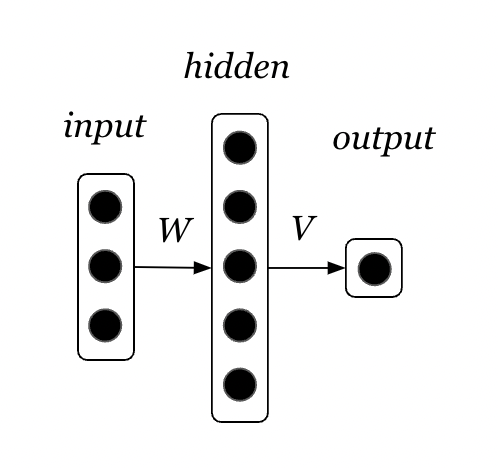
\includegraphics[width=0.3\textwidth]{images/fnn.png}
\caption{Example of a feedforward neural network}
\label{fig:fnn}
\end{figure}
A feedforward neural network consists of three parts: an input layer, one or more hidden layers, and an output layer. In a feedforward neural network, data only flows in one direction (forward) from input to output. Figure \ref{fig:fnn} shows an example of a feedforward neural network with one hidden layer. If the input to the network is represented by $x$, the hidden layer is computed by $f(W(x))$ and the output layer can be computed as $g(V(f(W(x))))$, where $W$, $V$ are the weights and $f$, $g$ are the activation functions. It has a simple structure, but it can be powerful in certain tasks.

\subsection{Recurrent Neural Network (RNN)}
\begin{figure}[ht]
\centering
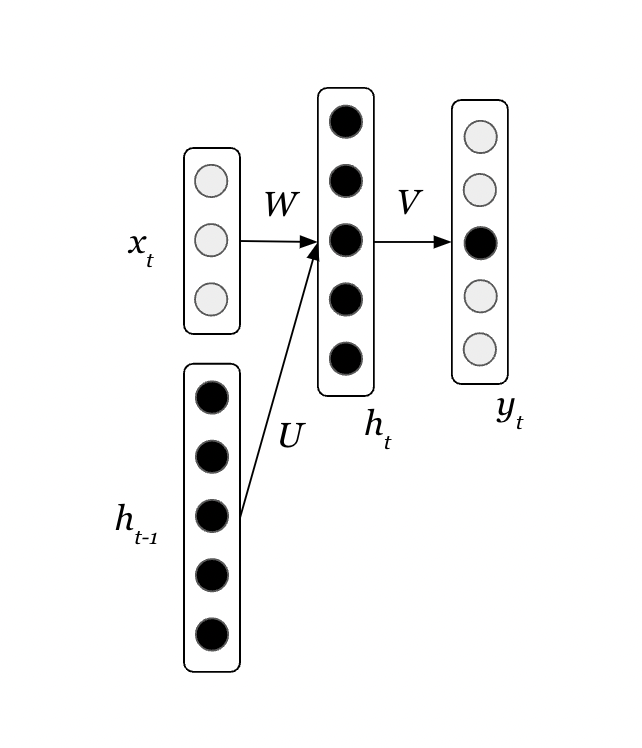
\includegraphics[width=0.25\textwidth]{images/rnn.png}
\caption{Example of a recurrent neural network (RNN)}
\label{fig:rnn}
\end{figure}
Recurrent neural networks are usually used to deal with sequences. They allow access to the input data as well as past data to compute the next state. As shown in Figure \ref{fig:rnn}, the hidden layer $h_t$ is computed using both input $x_t$ at time $t$ and the hidden state $h_{t-1}$ which contains the history information from time 0 to $t-1$. For each timestep $t$, the hidden state can be expressed as:
\[ h_t = Wx_t + Uh_{t-1} \]

And we can compute the probability of output at time $t$ by
\[ p(y_t) = \frac{e^{y_t}}{\sum_{i}e^{y_i}}\]


\subsection{Recursive Neural Network (RvNN)}
\begin{figure}[ht]
\centering
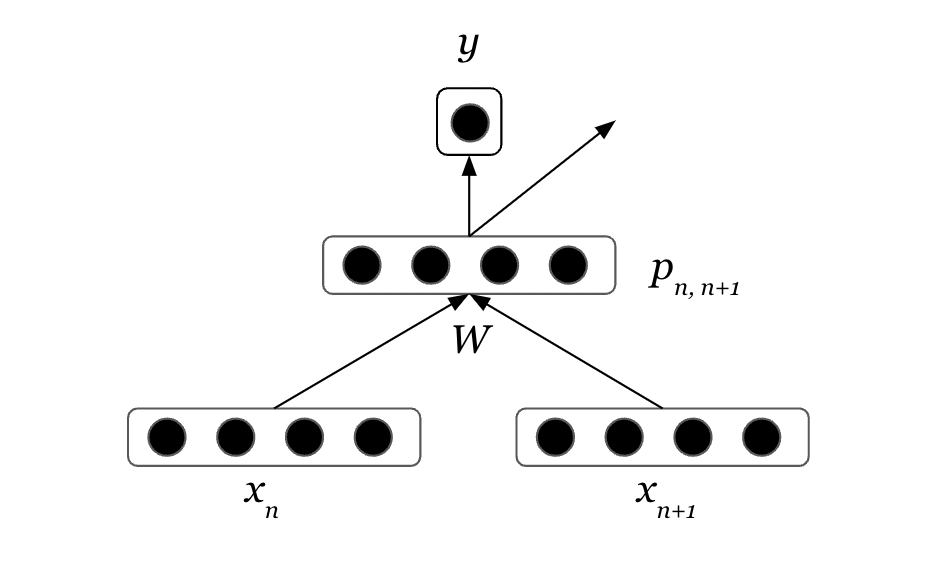
\includegraphics[width=0.5\textwidth]{images/rvnn.png}
\caption{Example of a recursive neural network (RvNN)}
\label{fig:rvnn}
\end{figure}
A recursive neural network has a tree-like structure. Figure \ref{fig:rvnn} illustrates an example of a basic RvNN architecture. The parent node representation is computed from its child nodes' representation as follows:
\[ p_{n, n+1} = f(W[x_n; x_{n+1}]) \]
where $f$ is the activation function. The same weight matrix $W$ would be applied recursively over the input.

\subsection{\texorpdfstring{Recursive Recurrent Neural Network (R\textsuperscript{2}NN)}{Recursive Recurrent Neural Network (R2NN)}}\label{section:r2nn_theory}
The R\textsuperscript{2}NN proposed by Liu et al.\cite{r2nn} combines the features of RvNN and RNN. It has a tree-like structure similar to RvNN, with recurrent vectors added to integrate global information. As shown in Figure \ref{fig:r2nn}, $s^{[l, m]}$ and $s^{[m, n]}$ is the representation of child nodes $[l, m]$ and $[m, n]$. The recurrent input vectors, $x^{[l, m]}$ and $x^{[m, n]}$ are added to the two child nodes respectively. They encode the global information, such as language model scores and distortion model scores. A third recurrent input vector $x^{[l, n]}$ is added to the parent node $[l, n]$. The parent node representation is computed as
\[ s_j^{[l, n]} = f(\sum_{i} \hat{x}_i^{[l, n]}w_{ji}) \]
where $\hat{x}$ is the concatenation of vectors $[x^{[l, m]}; s^{[l, m]}; x^{[m, n]}; s^{[m, n]}]$, and $f$ is the $HTanh$ function. The output, $y^{[l, n]}$, is computed as
\[ y^{[l, n]} = \sum_{j} ([s^{[l, n]}; x^{[l, n]}])_{j}v_j \]


\begin{figure}[ht]
\centering
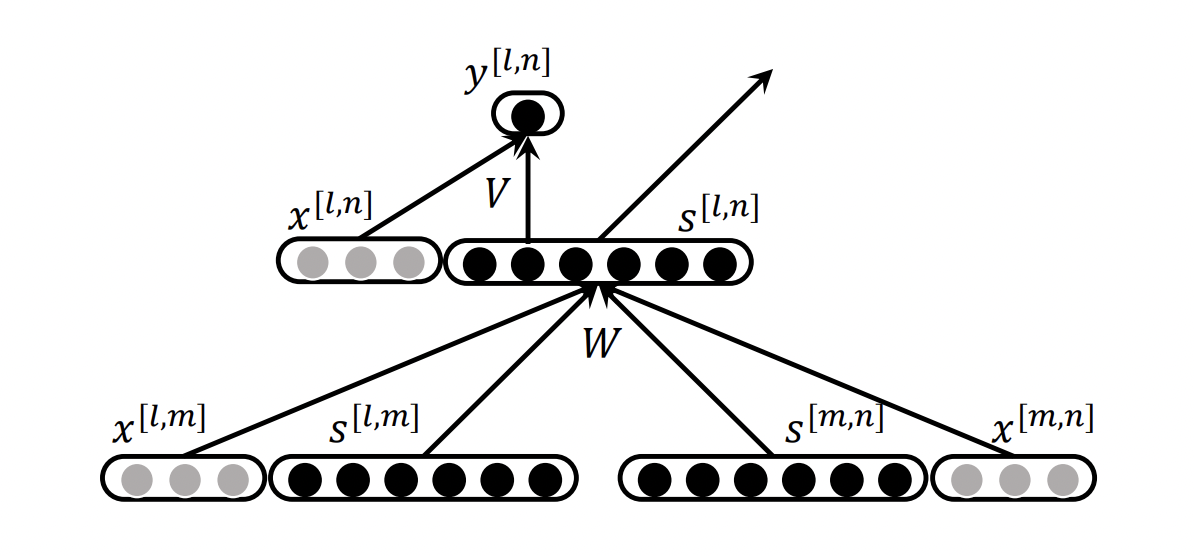
\includegraphics[width=0.6\textwidth]{images/r2nn.png}
\caption{Recursive recurrent neural network (Liu et al., 2014, p.1494)}
\label{fig:r2nn}
\end{figure}

\section{Requirement Analysis}\label{section:requirement}

Based on the Project Structure section from my project proposal, the following requirements have been identified:

\textbf{Data preprocessing}
\begin{itemize}
    \item Data should be prepared in a form that is accepted by Moses SMT and R\textsuperscript{2}NN SMT
    \item Preprocessing should be done carefully to avoid accidentally correcting some of the grammatical errors 
    
    \begin{itemize}
        \item E.g. capitalisation errors may go undetected if all sentences are lowercased during data preprocessing
    \end{itemize}
\end{itemize}

\textbf{Moses SMT for GEC}
\begin{itemize}
    \item A language model should be trained to model the probability of a given sentence being valid
    \item A translation model should be trained to construct a phrase translation table
    \item A reordering model should be trained to learn the reordering of phrases
    \item With the above three models and Moses decoder, a complete Moses SMT system should be built
\end{itemize}

\textbf{R\textsuperscript{2}NN SMT for GEC}

Following the R\textsuperscript{2}NN paper by Liu et al.\cite{r2nn},
\begin{itemize}
    \item Phrase pair embeddings (PPE) should be learned by building a one-hidden-layer neural network and a recurrent neural network
    \item A recursive recurrent neural network (R\textsuperscript{2}NN) should be built and used as a decoder
\end{itemize}

\textbf{Evaluation}
\begin{itemize}
    \item The performance of both SMT systems should be evaluated using F0.5 scores
\end{itemize}

\section{Choice of Tools}\label{section:tools}

\subsection{Programming Language}
Python is chosen to be the main programming language as it provides many libraries that are commonly used for natural language processing. For this project I used \texttt{python 3.8} and PyCharm as my IDE.

\subsection{Libraries}
\textbf{PyTorch} \\
The \texttt{PyTorch}\footnote{https://pytorch.org/} library is one of the most popular machine learning frameworks. There are other similar libraries (such as \texttt{TensorFlow}) but I find \texttt{PyTorch} tutorials are easier to follow.

\textbf{NumPy} \\
My project is likely to involve statistical processing. I would be using the \texttt{NumPy}\footnote{https://numpy.org/} library for this purpose.

\textbf{pandas} \\
\texttt{pandas}\footnote{https://pandas.pydata.org/} is a powerful library for processing tabular data. This would be used to manipulate phrase tables in my project.

\subsection{Dataset}
I used the \textbf{FCE v2.1} corpus\cite{yannakoudakis-etal-2011-new} in the BEA 2019 Shared Task as training, development and test data in this project. This is immediately downloadable from the website\footnote{https://www.cl.cam.ac.uk/research/nl/bea2019st/\#data}. The corpora have been standardised to be easily evaluated by ERRANT\cite{bryant-etal-2017-automatic}\cite{felice-etal-2016-automatic}. ERRANT is a toolkit used to annotate parallel data and compare a hypothesis against a reference to produce various evaluation metrics including F0.5 score. I may request other corpora as an extension of my project.

For language model training, I used the \textbf{One Billion Word} dataset\cite{one-billion-word}. This is a dataset used for language modeling and is available on GitHub\footnote{https://github.com/ciprian-chelba/1-billion-word-language-modeling-benchmark}.

\subsection{Version Control and Backup}
Git was used for version control. The entire project, including all the written code and my dissertation, was pushed to GitHub regularly to protect against machine failures.


\chapter{Implementation}
\textit{This chapter concerns the implementation of the two major systems in this project. Section \ref{section:setup} describes how I set up training data. In section \ref{section:moses_baseline} and \ref{section:r2nn} I present the implementation of a baseline Moses SMT system and an R\textsuperscript{2}NN SMT system respectively. In section \ref{section:repo} I give an overview of my code repository.}

Since the main purpose of this project is to compare the performance of an R\textsuperscript{2}NN decoder against a Moses decoder, the R\textsuperscript{2}NN system should use the same language model, translation model and reordering model as Moses. For the translation model, the R\textsuperscript{2}NN paper\cite{r2nn} proposed a \textit{translation confidence based phrase pair embedding} (TCBPPE) to be used with the R\textsuperscript{2}NN decoder. The TCBPPE was based on a phrase table produced by the Moses translation model. In the end, the R\textsuperscript{2}NN decoder made use of the language model scores, translation model scores and reordering model scores from Moses and TCBPPE to find the best translation candidate.

\section{Setup}\label{section:setup}

\subsubsection{FCE Dataset}

The FCE dataset contains 28327 sentences in the training set, 2187 sentences in the development set and 2695 sentences in the test set. All the files were provided in m2 format. However, Moses requires parallel data which is aligned at the sentence level. An example\footnote{This means that for source sentence S, the word at position 8 to 9 (\textit{at}) should be corrected to the word \textit{to}.} taken from the m2 file looks like this:

\texttt{S} \textit{Her friend Pat had explained the whole story at her husband .}\\
\texttt{A 8 9|||R:PREP|||to|||REQUIRED|||-NONE-|||0}

The m2 format needs to be converted to sentence-aligned data to be used by Moses. A script\footnote{https://www.cl.cam.ac.uk/research/nl/bea2019st/data/corr\_from\_m2.py} was provided on the BEA 2019 Shared Task website to generate the corrected text from an M2 file. Based on this script, I wrote some Python code to extract source sentences and corrected sentences into two separate files which are aligned at the sentence level.

For the example above, the source sentence should be

\textit{Her friend Pat had explained the whole story at her husband .}

and the corrected sentence should be

\textit{Her friend Pat had explained the whole story to her husband .}

\subsubsection{One Billion Word Dataset}

I downloaded the One Billion Word dataset for language model training. However, the files were too large (about 18.2 GB) to be handled by my machine. Since the dataset consists of fifty files, I decided to randomly choose 10 files from them and concatenated these files to be used in language model training. 


\section{Moses Baseline} \label{section:moses_baseline}

\begin{figure}[ht]
\centering
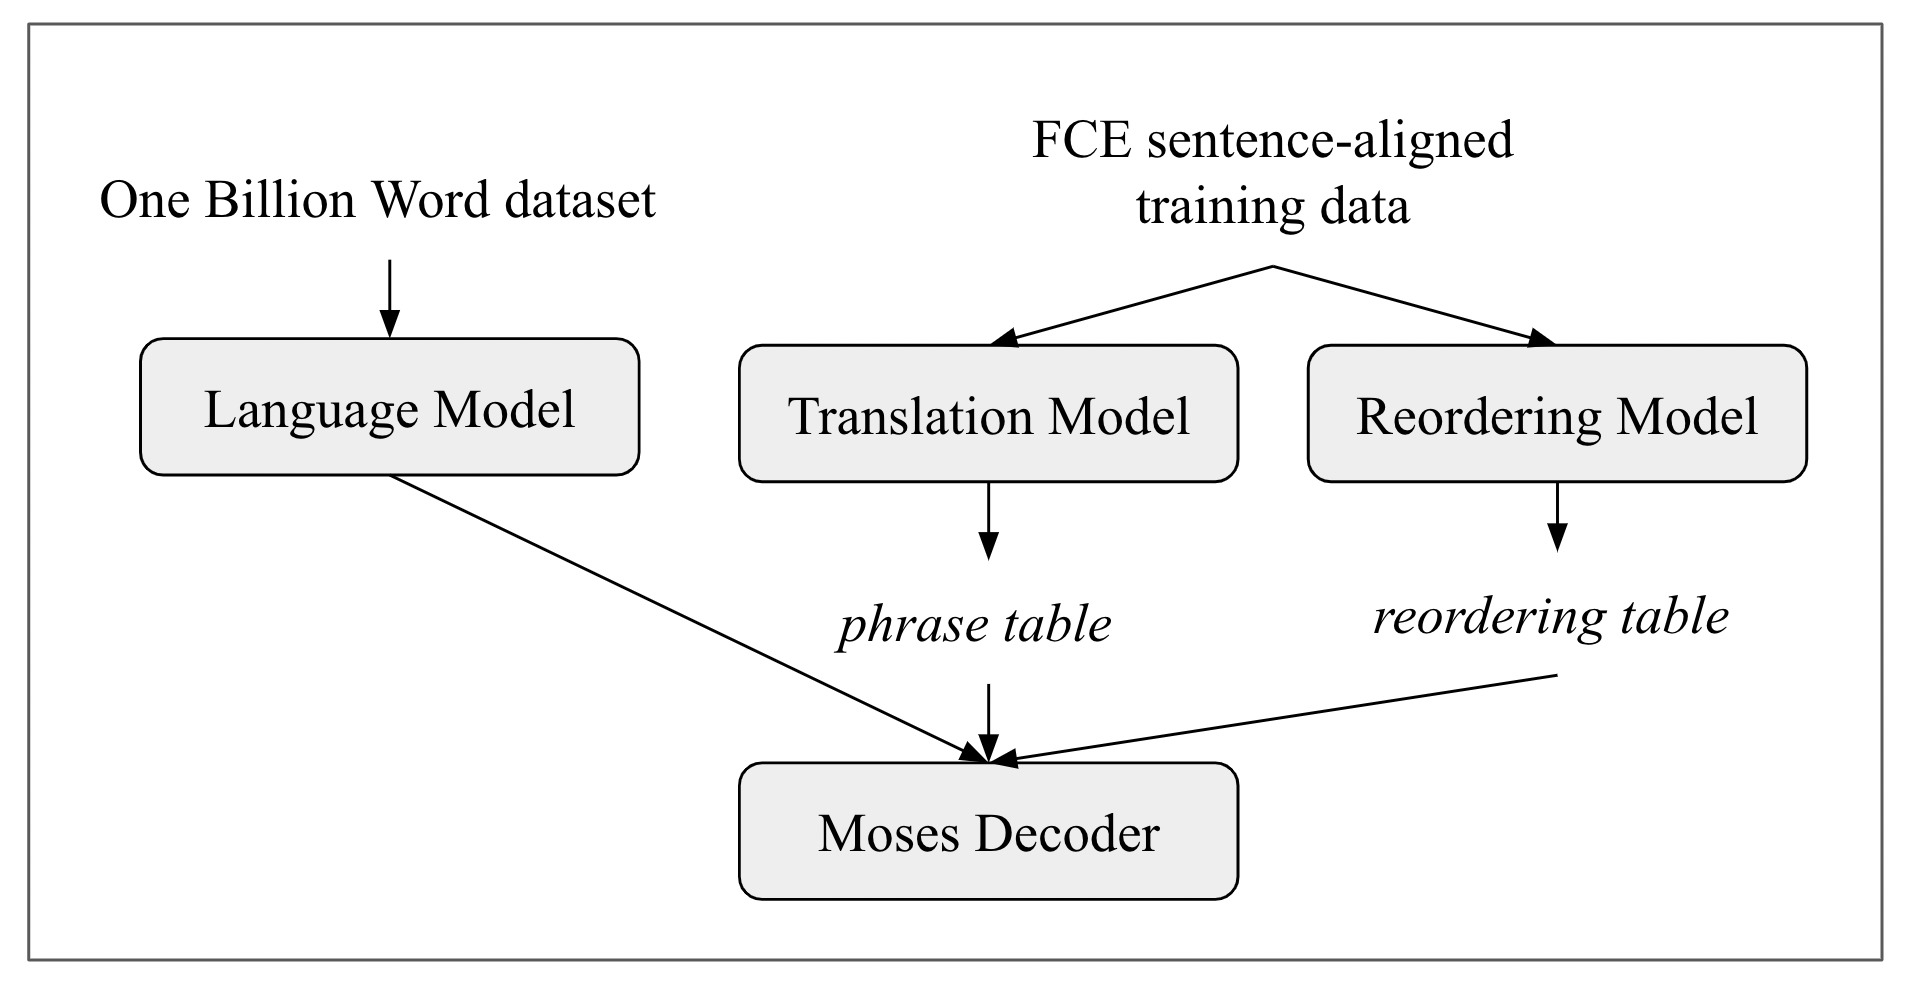
\includegraphics[width=0.8\textwidth]{images/moses_pipeline.png}
\caption{Overview of Moses SMT (training)}
\label{fig:moses_pipeline}
\end{figure}

To build a baseline Moses SMT system, three models need to be trained: a language model, a translation model and a reordering model.

\subsection{Language Model}\label{section:moses_lm}
The One Billion Word dataset is used for language model training. In the R\textsuperscript{2}NN paper, a 5-gram language model is used. Here, I used KenLM which came with Moses installation to train a 5-gram language model. As discussed in section \ref{section:SMT_system}, this means that the language model would look at 4 words in the past. After training, the language model is able to compute a total score for any given sequence of words. The score represents the log probability of this sequence and would be used as the language model score (LM score) later on. The example below shows that our trained language model assigns a higher score to a valid English sentence compared to incorrect English sentences.

\begin{center}
\begin{tabular}{ c | c }
 \textbf{Sentence} & \textbf{LM score} \\ 
 \hline
 \textit{I have an apple .} & $-9.682597$ \\ 
 \textit{I have apple .} & $-11.434978$ \\ 
 \textit{I has apple .} & $-13.841325$ 
\end{tabular}
\end{center}

\subsection{Translation Model and Reordering Model}\label{section:moses_tm}
The translation model is trained with FCE sentence-aligned data. There are three components in translation model training: word alignment, phrase extraction and scoring. Word alignment is obtained using GIZA++, a toolkit to train word alignment models. Phrases are then extracted from our training files and a phrase table is produced. A distance-based reordering model is also built, and a reordering table is created. 

Table \ref{table:phrase_table} shows part of the phrase table generated by Moses\footnote{In the actual file, columns are separated by $\vert\vert\vert$}. Each phrase pair from the training data has an unique entry in the phrase table. Four translation scores are computed for every phrase pair, namely inverse phrase translation probability \texttt{(target $\rightarrow$ source)}, inverse lexical weighting, direct phrase translation probability \texttt{(source $\rightarrow$ target)}, and direct lexical weighting. The phrase table also contains the alignment between the source phrase and the target phrase. The column named `counts' contains three numbers. The first is the number of times the target phrase appeared in the training target file, \texttt{count(target)}. The second is the frequency of the source phrase in the training source file, \texttt{count(source)}. The third is the number of times that the source phrase is mapped to the target phrase, \texttt{count(source $\rightarrow$ target)}.

\begin{table}[ht]
\centering
\begin{tabular}{ |c|c|c|c|c| } 
 \hline
 source & target & scores & alignment & counts \\ [0.5ex] 
 \hline
 As we & As we & 1 0.901657 0.846154 0.90511 & 0-0 1-1 & 11 13 11\\
 As we & We & 0.00115075 1.68879e-05 0.0769231 0.0153198 & 1-0 & 869 13 1\\
 As we & as we & 0.0212766 0.00117032 0.0769231 0.00482726 & 0-0 1-1 & 47 13 1\\
 \hline
\end{tabular}
\caption{Phrase table from Moses}
\label{table:phrase_table}
\end{table}

After training, a configuration file named \texttt{moses.ini} is generated. By modifying the configuration file, we can change the language model, translation model and reordering model used by Moses decoder.


\section{\texorpdfstring{R\textsuperscript{2}NN}{R2NN} SMT}\label{section:r2nn}

The R\textsuperscript{2}NN SMT model consists of three parts: translation confidence based phrase pair embedding (TCBPPE), global features, and an R\textsuperscript{2}NN decoder. Section \ref{section:TCBPPE_sparse} and \ref{section:TCBPPE_rnn} presents implementation and training of two neural networks for sub-components of TCBPPE, and section \ref{section:TCBPPE} demonstrates how they are combined together to be phrase pair embedding. Section \ref{section:global_features} describes how I obtained global features, the recurrent input vector to R\textsuperscript{2}NN model. Finally, I discuss my implementation of an R\textsuperscript{2}NN decoder using TCBPPE and global features in section \ref{section:r2nn_model}.

\begin{figure}[ht]
\centering
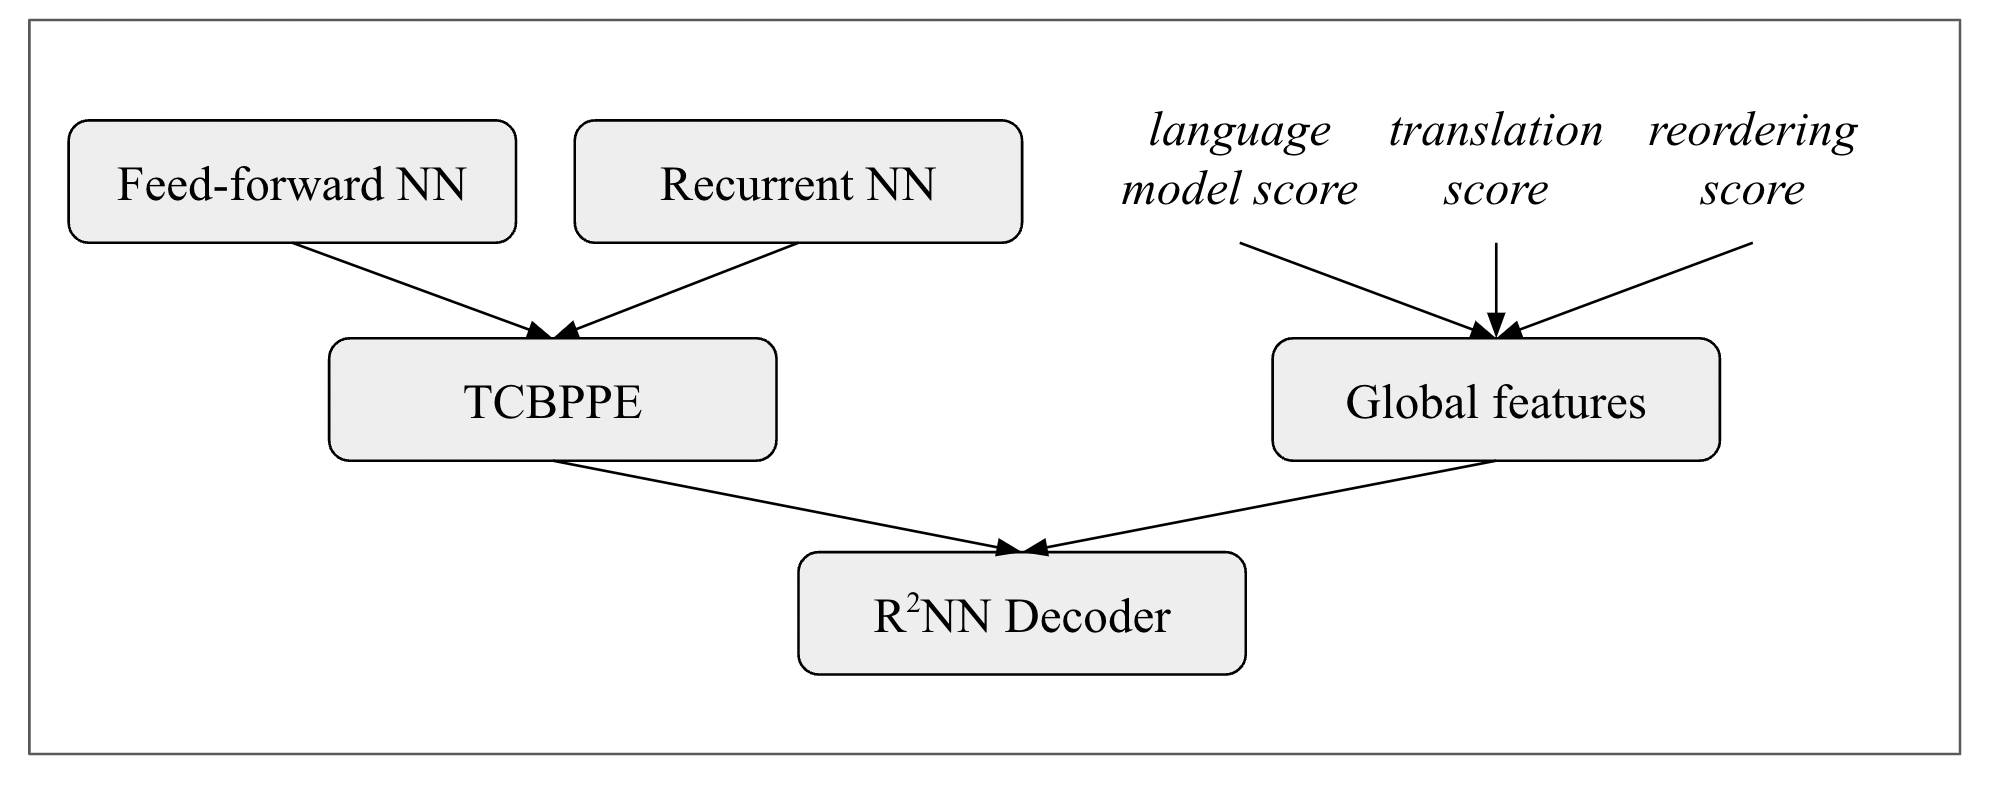
\includegraphics[width=1\textwidth]{images/r2nn_pipeline.png}
\caption{Overview of R\textsuperscript{2}NN SMT (training)}
\label{fig:r2nn_pipeline}
\end{figure}

\subsubsection{TCBPPE}
A phrase pair embedding is a vector representation which encodes the meaning of a phrase pair. This was used as the \textbf{representation vector} in R\textsuperscript{2}NN model. 

Liu et al.\cite{r2nn} argued that the phrase pair embedding should capture the translation relationship between phrase pairs at phrase level. They presented a \textbf{translation confidence based phrase pair embedding} (TCBPPE) method and demonstrated that it was better than simply taking the average of the embedding of words. Their phrase pair embedding is split into two parts: translation confidence with sparse features (section \ref{section:TCBPPE_sparse}) and translation confidence with recurrent neural network (section \ref{section:TCBPPE_rnn}). These two embeddings were obtained separately and then concatenated together (section \ref{section:TCBPPE}) to be used as the representation vector of each phrase pair.

\subsubsection{Global features}
The global features encode global information that cannot be generated by child representations. This was used as the \textbf{recurrent input vector} in R\textsuperscript{2}NN model. 

In the paper\cite{r2nn}, three scores are selected to be the global features: language model scores, translation scores and reordering scores. These scores are concatenated together to be used as the recurrent vector of each phrase pair (section \ref{section:global_features}).

\subsubsection{R\textsuperscript{2}NN decoder}
A recursive recurrent neural network (R\textsuperscript{2}NN) was used as a decoder to find the best translation candidate. For an input sentence, the decoder would construct a tree based on phrases in the sentence. An output score was computed based on TCBPPE, global features and the structure of the tree. The translation candidate that gives the highest score would be the best translation candidate.

\subsection{TCBPPE: Sparse Features} \label{section:TCBPPE_sparse}

We use a one-hidden-layer feedforward neural network to obtain TCBPPE using sparse features as described in the paper\cite{r2nn}. The structure of the network is shown in Figure \ref{fig:one_hidden_layer}, with the size of the hidden layer set to 20. To train the network, we need to encode training data as a sparse matrix. Each of the top 200,000 frequent phrase pairs in the \textit{phrase table} is a feature, and a special feature is added to represent all the infrequent phrase pairs. For every sentence in the training data, we obtain a binary vector of length 200,001. It only contains 1s in the position where the phrase pair exists in the sentence.

\begin{figure}[ht]
\centering
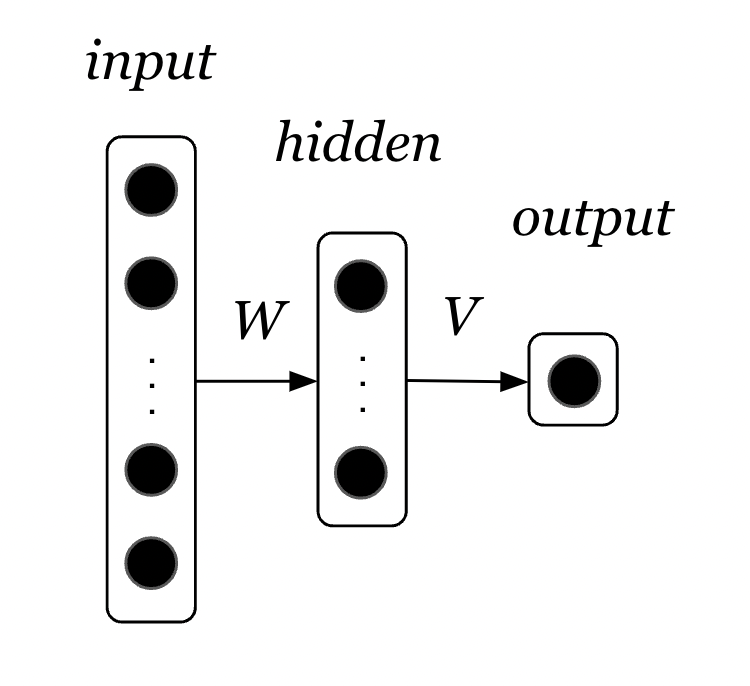
\includegraphics[width=0.3\textwidth]{images/one_hidden_layer.png}
\caption{Structure of one-hidden-layer feedforward neural network}
\label{fig:one_hidden_layer}
\end{figure}

By training the network, we obtain a hidden matrix $W$ of size 200,001 by 20. $W$ would be used as the \textbf{phrase pair embedding matrix for sparse features} (\texttt{ppe\_sparse}). The goal is to find the $W$ that gives the best phrase pair embedding.

In the following sections, I will discuss the method used to obtain the top 200,000 phrase pairs since it is an essential component in encoding training data. I will describe how I encoded training data into a sparse matrix with the help of top phrase table. Finally I will present the result of my network after training and how I obtained the first part of TCBPPE with sparse features.

\subsubsection{Obtain the top phrase table}
Firstly, we need to obtain the 200,000 most frequent phrase pairs from the \textit{phrase table} given by Moses SMT (section \ref{section:moses_tm}). Recall in Table \ref{table:phrase_table}, three counts were given in the Moses phrase table: the target phrase frequency, the source phrase frequency, and the phrase pair frequency. I use the \texttt{pandas} library to read the table and perform sorting on these counts. The frequency of each phrase pair appeared in the training data is sorted in descending order. If multiple phrase pairs have the same frequency, they were further sorted by target phrase frequency and source phrase frequency in descending order. After sorting, we keep the top 200,000 rows of the table to be the \textit{top phrase table}.

\subsubsection{Encode training data}
\begin{figure}[ht]
\centering
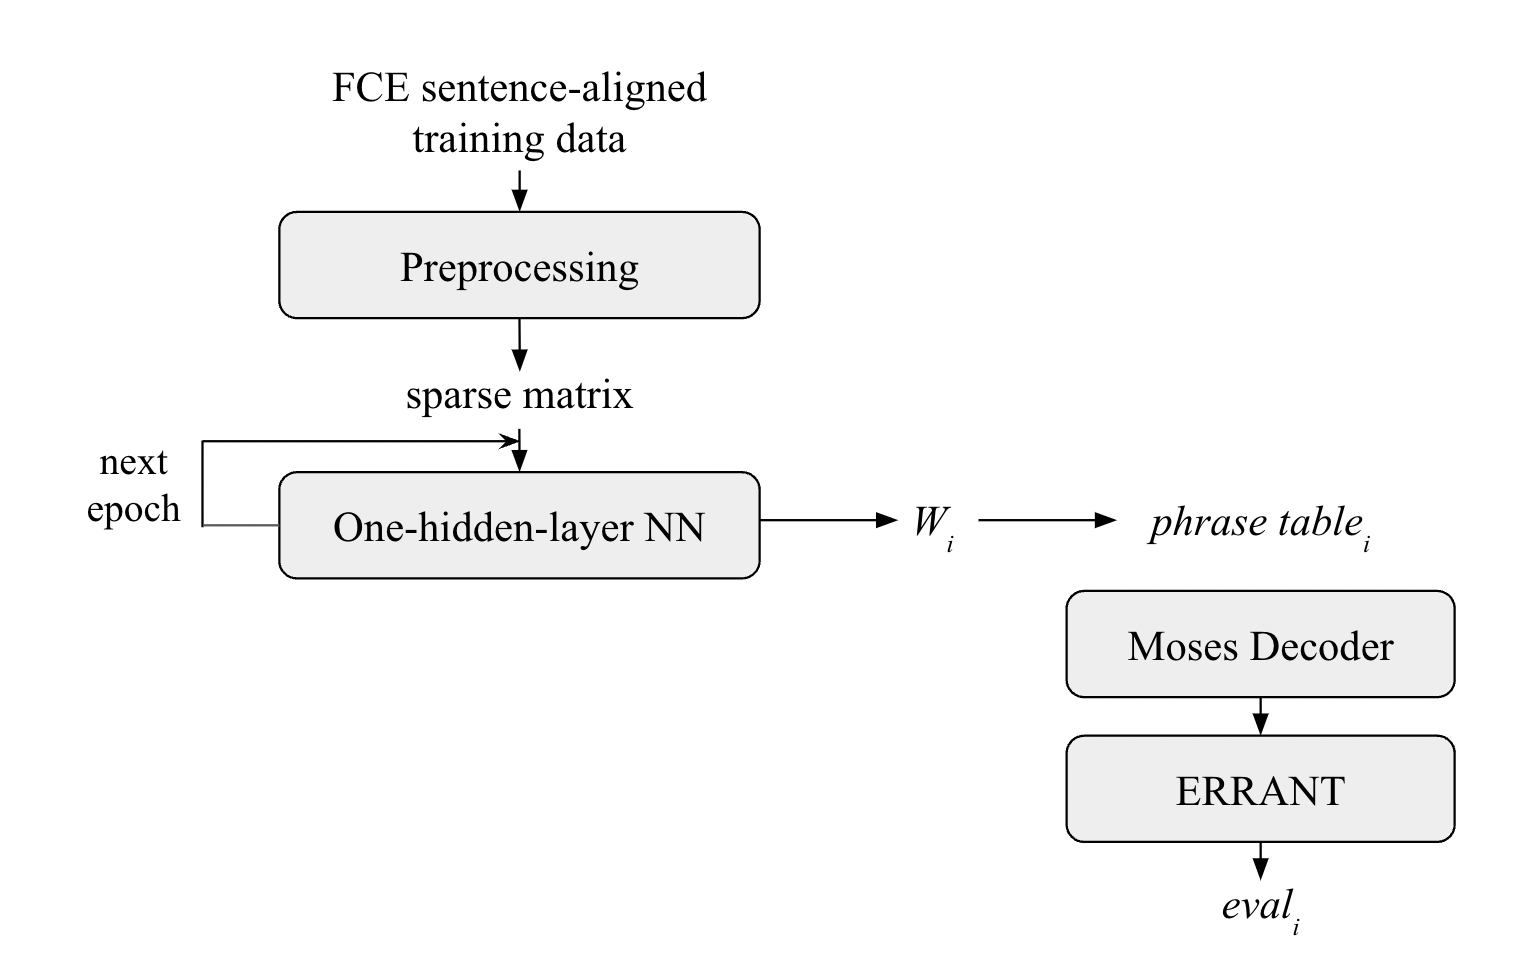
\includegraphics[width=0.8\textwidth]{images/sparse_pipeline.png}
\caption{Training pipeline of the one-hidden-layer feedforward neural network}
\label{fig:sparse_pipeline}
\end{figure}

The next step is to encode our training data as a sparse matrix. Consider the following sentence pair:

\textbf{Source sentence}
\textit{What she would do ?}

\textbf{Target sentence}
\textit{What would she do ?}

The encoded vector (of length 200,001) for this sentence pair would look like this:

\textbf{Encoded vector}
\texttt{[$\underset{0}{0}, \ldots, \underset{39}{1}, \ldots$]}

A 0 at position 0 means that the most frequent phrase pair does not exist in the sentence pair. A 1 at position 39 means that the 40\textsuperscript{th} most frequent phrase pair exists in the sentence pair. If the sentence pair contains a phrase pair that is not in the top 200,000 most frequent pairs, it would contain a 1 at position 200,000.

One problem with this is that the resulting matrix is going to be a sparse matrix of size \texttt{training size} by 200,001. To save memory, instead of storing the whole matrix, the position indices of 1s in the vector are stored in a file named \texttt{phrase\_pair\_id} (i.e. the phrase pair ids used in each sentence pair). When loading the sentence pairs as training data, it is easy to retrieve the sparse matrix from \texttt{phrase\_pair\_id}.

Next, we need to get the expected output for each input sentence pair. Since the TCBPPE encodes translation model information, it is reasonable to use the translation scores from the Moses translation model. For each sentence pair $S\textrm{-}T$ containing phrase pairs $p_1, p_2, ..., p_n$, the expected output score is computed by
\[ score_{S\textrm{-}T} = \frac{\sum_n c_{p_n}}{n} \]
where $c_{p_n}$ is the average translation score for phrase pair $p_n$.

\subsubsection{Training the one-hidden-layer neural network}
After encoding the training dataset, we can start training the neural network. Since the goal is to obtain the hidden matrix $W$ that gives the best phrase pair embedding, we evaluated the performance of $W$ after every epoch, i.e. one cycle of processing all the data in the training set, to decide when to stop training.

$W$ is evaluated by updating the Moses phrase table. Each row in $W$ is used as the phrase pair embedding (ppe) for the phrase pair it represents. We then add the ppe to the phrase table as an additional feature. Then we pass the updated phrase table to the Moses decoder and use ERRANT to evaluate the performance. Figure \ref{fig:sparse_pipeline} demonstrates the training pipeline of the neural network.

\begin{figure}[ht]
\centering
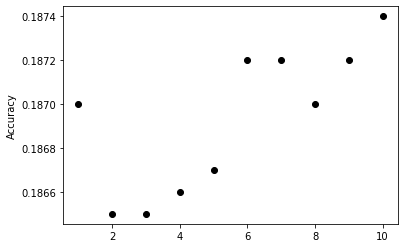
\includegraphics[width=0.6\textwidth]{images/sparse_acc.png}
\caption{Plot of accuracy given by ERRANT scorer against number of epochs}
\label{fig:sparse_acc}
\end{figure}

\begin{figure}[ht]
\centering
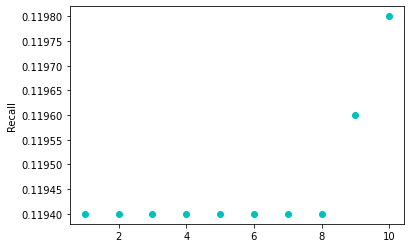
\includegraphics[width=0.6\textwidth]{images/sparse_rec.png}
\caption{Plot of recall given by ERRANT scorer against number of epochs}
\label{fig:sparse_rec}
\end{figure}

\begin{figure}[ht]
\centering
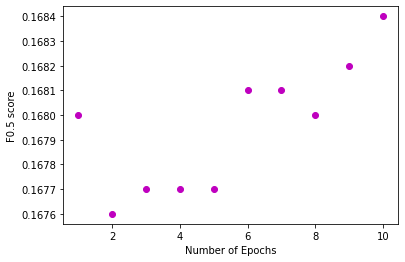
\includegraphics[width=0.6\textwidth]{images/sparse_f.png}
\caption{Plot of $F_{0.5}$ score given by ERRANT scorer against number of epochs}
\label{fig:sparse_f}
\end{figure}

Figure \ref{fig:sparse_acc}, \ref{fig:sparse_rec} and \ref{fig:sparse_f} shows how accuracy, recall and $F_{0.5}$ score change as the number of epochs increases. Training for 10 epochs gives the highest accuracy, recall as well as $F_{0.5}$ score. For this reason, we used the $W$ after epoch 10 as the first part of the TCBPPE (\texttt{ppe\_sparse}). 

\subsection{TCBPPE: Recurrent Neural Network (RNN)} \label{section:TCBPPE_rnn}

\begin{figure}[ht]
\centering
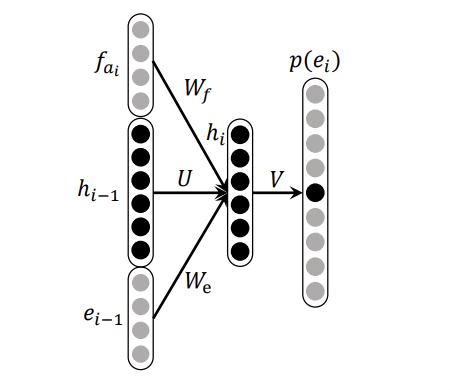
\includegraphics[width=0.4\textwidth]{images/rnn_ppe.png}
\caption{Recurrent neural network for translation confidence (Liu et al., 2014, p.1497)}
\label{fig:rnn_ppe}
\end{figure}

The other part of TCBPPE is a \textbf{translation confidence score} generated by a recurrent neural network (RNN). The structure of the RNN used in the paper\cite{r2nn} is shown in Figure \ref{fig:rnn_ppe}, where $e_i$ is the source word embedding, and $f_{a_i}$ is the word embedding of the target word which is aligned to $e_i$. The translation confidence score from source $s$ to target $t$ is given by
\[ T_{S2T}(s, t) = \sum_{i} \log p(e_i|e_{i-1}, f_{a_i}, h_i)\]

In the following sections I will describe the preprocessing of training data. I will illustrate my implementation of the RNN structure as shown in the paper\cite{r2nn} and how I trained the neural network to obtain the \textbf{translation confidence score} (\texttt{ppe\_rnn}) of the TCBPPE.

\subsubsection{Preprocess training data}
Firstly, we need to decide what to use for word embedding. There are several popular pre-trained word embedding models available, such as GloVe\footnote{https://nlp.stanford.edu/projects/glove/} and fastText\footnote{https://fasttext.cc/docs/en/crawl-vectors.html}. I used the fastText pre-trained models because fastText is based on character n-grams, whereas GloVe takes a word to be the smallest unit. For the task of Grammatical Error Correction, it is likely that OOV (out of vocabulary) words will occur in the source (such as misspelled words). fastText can easily generate word embedding for those unseen words based on character n-grams.

Next, we construct a PyTorch dataset from the FCE training data. Consider a sentence pair with 
\[s_1s_2\dots s_m\]
as a source sentence of $m$ words, and
\[t_1t_2\dots t_n\]
as a target sentence of $n$ words. We use fastText to obtain a word embedding for each word in source and target. Let $e_i$ be the word embedding for $t_i$ in target, $e_{i-1}$ be the word embedding for $t_{i-1}$ i.e. the previous word in target, $f_{a_i}$ be the word embedding for $s_j$ which is the word in source that is aligned to $t_i$. The input to the RNN would be $e_{i-1}$ and $f_{a_i}$, and the output would be the probability distribution of word $e_i$. 

For special cases when either $e_{i-1}$ does not exist (e.g. if $e_i$ is the word embedding of the first word in the sentence) or when there is no $f_{a_i}$ if $e_i$ is not aligned to any word, a zero vector was used as the word embedding instead to avoid None Type error.

\subsubsection{Training RNN}

\begin{figure}[ht]
\centering
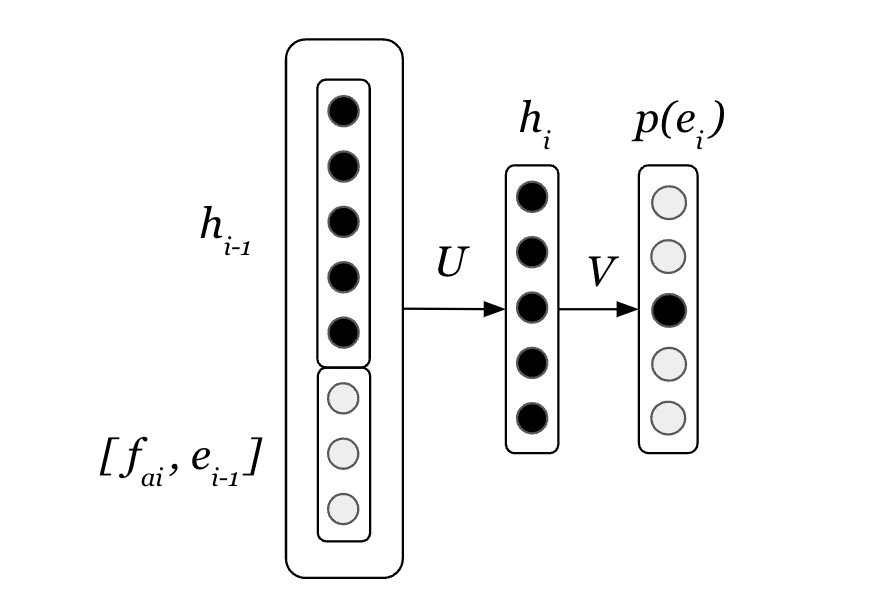
\includegraphics[width=0.45\textwidth]{images/rnn_code.png}
\caption{My implementation of RNN according to Figure \ref{fig:rnn_ppe}}
\label{fig:rnn_code}
\end{figure}

Figure \ref{fig:rnn_code} shows the structure of my implementation of RNN, following the paper\cite{r2nn}. The size of the word embedding is set to 50 to avoid memory issues, and the size of the hidden layer is set to 100. The input layer is a concatenation of $f_{a_i}$, $e_{i-1}$ and the hidden layer. A log softmax layer is applied at the end to convert output to a categorical probability distribution, hence the size of the output layer should be the number of unique words in the training data.

The RNN was trained for 3 epochs and the model state was stored. Using the trained network, we compute $T_{S2T}(s, t)$ for each phrase pair $(s, t)$ in the top phrase table by
\[ T_{S2T}(s, t) = \sum_{i} \log p(e_i|e_{i-1}, f_{a_i}, h_i)\]
for $e_i$ in source phrase and $f_{a_i}$ in target phrase. This computed score was used as the other part of TCBPPE for the phrase pair $(s, t)$. After computing a score for all the phrase pairs in the top table, we obtain \texttt{ppe\_rnn} of size 200,000 by 1.

\subsection{TCBPPE}\label{section:TCBPPE}
In section \ref{section:TCBPPE_sparse}, we obtained the first part of TCBPPE with sparse features, resulting in a matrix \texttt{ppe\_sparse} of size 200,001 by 20. In section \ref{section:TCBPPE_rnn}, we obtained the second part of TCBPPE using a recurrent neural network, which gives a matrix \texttt{ppe\_rnn} of size 200,000 by 1. To get the full phrase pair embedding, we need to concatenate \texttt{ppe\_sparse} and \texttt{ppe\_rnn} together to obtain a matrix of size 200,001 by 21, where the size of phrase pair embedding for each pair is of length 21. To achieve that, we need to append an element to the end of \texttt{ppe\_rnn} to make it of size 200,001 by 1. I used value 0 for this purpose. The resulting matrix becomes the \textit{representation vector} for all the phrase pairs, with the top 200,000 rows being the \textit{representation vector} for the top 200,000 phrase pairs and the 200,001\textsuperscript{th} row being the \textit{representation vector} for all the infrequent phrase pairs.

\subsection{Global Features} \label{section:global_features}
In the paper\cite{r2nn}, three features are proposed to be used as global features, namely language model score, translation model score and reordering model score. Language model scores can be obtained by querying the language model from Moses SMT (section \ref{section:moses_lm}). Translation model scores are accessible from the Moses phrase table (section \ref{section:moses_tm}). However, although a reordering table was created by Moses after training, it is unclear what each score means and Moses documentation did not give details of the reordering score components. In addition, Junczys-Dowmunt and Grundkiewicz disabled reordering in their experiment with phrase-based SMT in the paper\cite{junczys-dowmunt-grundkiewicz-2016-phrase} as word order errors are fairly rare in GEC. Hence, the reordering scores are omitted and only translation model score and language model score were used as global features in my implementation of R\textsuperscript{2}NN decoder.

For each phrase pair in the phrase table, we need to obtain a \textbf{language model score} and a \textbf{translation model score}. The language model score (LM score) is given by the trained 5-gram KenLM language model described in section \ref{section:moses_lm}. We pass the target phrase in each phrase pair to the language model, and the resulting LM score is saved for this phrase pair. Four scores were calculated by Moses in the phrase table (section \ref{section:moses_tm}). In order to make use of all four features, the translation model score is calculated by taking average of the four scores for each phrase pair.

Finally, we concatenate the language model score and the translation model score to be a vector of length 2 and this was used as the \textit{recurrent input vector} to R\textsuperscript{2}NN model.

\subsection{\texorpdfstring{R\textsuperscript{2}NN}{R2NN} Decoder} \label{section:r2nn_model}
In the following sections, I will describe how I prepare the training data for R\textsuperscript{2}NN using forced decoding. I will present my implementation of R\textsuperscript{2}NN by extending an implementation of recursive neural network. Finally, I will discuss how I trained the recursive recurrent neural network.

\subsubsection{Prepare training data}
Following the R\textsuperscript{2}NN paper\cite{r2nn}, forced decoding was used to generate positive samples. Forced decoding is a technique used to find out how the model derives a translation. We can perform forced decoding with Moses by constraining the output of the decoder to only be the reference sentences (i.e. the target sentences in FCE training dataset). This produces a file which contains the rules/phrases used in the translation from source sentences to target sentences. From this file, we need to obtain
\begin{itemize}
  \item the phrase pairs used in each sentence pair, and
  \item the scores associated with the translation.
\end{itemize}

Below is an example taken from the forced decoding output file.
\begin{lstlisting}[breaklines]
    TRANSLATION HYPOTHESIS DETAILS:
             SOURCE: [0..4] Dear Sir or Madam ,
      TRANSLATED AS: Dear Sir or Madam ,
      WORD ALIGNED: 0-0 1-1 2-2 3-3 4-4 
    SOURCE/TARGET SPANS:
      SOURCE: 0-1-2-3-4
      TARGET: 0-1-2-3-4
    SCORES (UNWEIGHTED/WEIGHTED): core=(0.000,-5.000,1.000,-0.108,...,-31.078,0.000)
\end{lstlisting}

We extract the following information from this translation:

\textbf{Phrase pairs used}\\
\textit{Dear Sir or Madam , $\rightarrow$ Dear Sir or Madam ,}

\textbf{Scores}\\
\textit{(0.000, -5.000, 1.000, -0.108, ..., -31.078, 0.000)}

The phrase pairs used in this translation indicate how the source sentence is split into phrases. The list of source phrases would be the input to the R\textsuperscript{2}NN decoder. The scores are the log probabilities computed from features used in the decoder. We sum up the scores to be the \textit{forced decoding score}, and this would be the expected output score for this translation.

\subsubsection{Building an \texorpdfstring{R\textsuperscript{2}NN}{R2NN}}
\begin{figure}[ht]
\centering
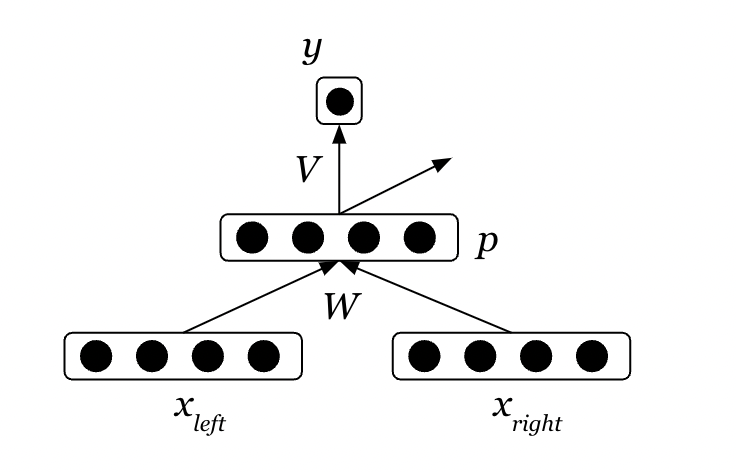
\includegraphics[width=0.45\textwidth]{images/rvnn_imple.png}
\caption{My implementation of a recursive neural network}
\label{fig:rvnn_imple}
\end{figure}

Since no implementation of an R\textsuperscript{2}NN is publicly available, I developed my own version as follows. 

As demonstrated in Figure \ref{fig:r2nn}, a recursive recurrent neural network has a tree-like structure. I started with building a recursive neural network (RvNN) with the structure shown in Figure \ref{fig:rvnn_imple}, where $x_{left}$ and $x_{right}$ are the representation of the left child node and right child node. The parent node representation is computed as 
\[p = W([x_{left}; x_{right}])\]

where $[a;b]$ denotes concatenation of vector $a$ and $b$. The output score is computed as
\[y = V(p)\]

A separate class, \texttt{TreeNode}, is defined to make use of the above RvNN. This class provides a method named $greedy\_tree$ which constructs a tree from a list of leaf nodes based on the output score from the RvNN. The algorithm used in $greedy\_tree$ is demonstrated in Algorithm \ref{alg:tree}.

\begin{algorithm}
\caption{An algorithm which constructs a tree using a greedy method}\label{alg:tree}
\begin{algorithmic}
\State $leafs \gets$ $list$ $of$ $leaf$ $representation$
\State $n \gets size(leafs)$
\While{$n \ge 2$}
    \State $max$ $score\gets -\infty$
    \State $max$ $hypothesis\gets None$
    \State $index\gets None$
    \For{$i\gets 1, n$}
        \State $hypothesis\gets new$ $TreeNode$
        \State $hypothesis.left\gets leafs[i-1]$
        \State $hypothesis.right\gets leafs[i]$
        \State $score\gets RvNN(hypothesis)$
        
        \If{$score > max$ $score$}
            \State $max$ $score\gets score$
            \State $max$ $hypothesis\gets hypothesis$
            \State $index\gets i$
        \EndIf
    \EndFor
    \State $leafs[index-1:index+1]\gets [max$ $hypothesis]$
\EndWhile
\end{algorithmic}
\end{algorithm}

In principle, given a list of leaf node representations, this algorithm constructs a tree by finding the parent that gives the highest score computed by RvNN and repeat until only one tree node is left, which becomes the root node of the constructed tree. The final output score assigned to this tree can be obtained by passing the tree to RvNN.

\begin{figure}[ht]
\centering
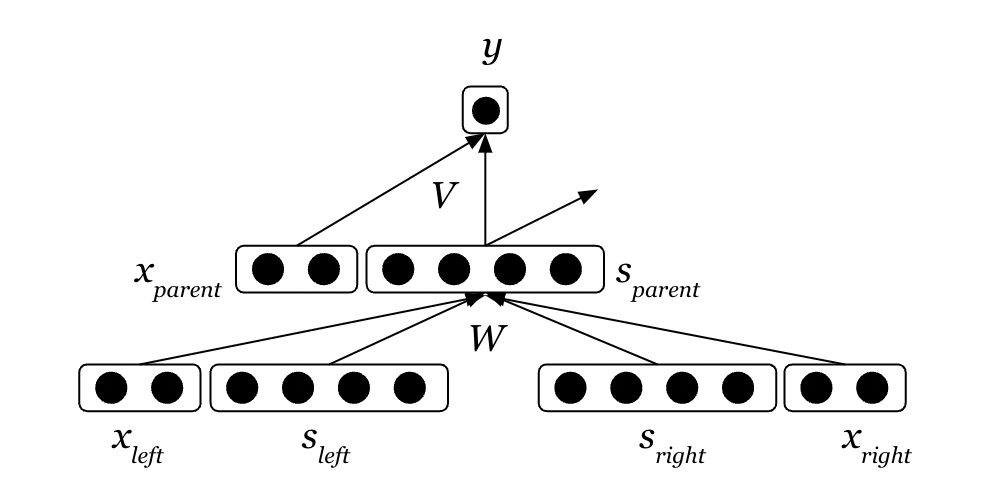
\includegraphics[width=0.6\textwidth]{images/r2nn_imple.png}
\caption{My implementation of a recursive recurrent neural network}
\label{fig:r2nn_imple}
\end{figure}

My implementation of a recursive recurrent neural network R\textsuperscript{2}NN was based on the structure of \texttt{RvNN} and \texttt{TreeNode}. Recall in section \ref{section:r2nn_theory} we discussed the structure of an R\textsuperscript{2}NN\cite{r2nn}. For each node, we have a \textit{representation vector} and a \textit{recurrent input vector}. The representation vector is the translation confidence based phrase pair embedding (TCBPPE) which was discussed in section \ref{section:TCBPPE_sparse}, \ref{section:TCBPPE_rnn} and \ref{section:TCBPPE}. The recurrent input vector encodes global information and it was addressed in section \ref{section:global_features}. 

Figure \ref{fig:r2nn_imple} shows my implementation of an R\textsuperscript{2}NN. $s_{left}$ and $s_{right}$ is the TCBPPE for left phrase pair and right phrase pair respectively. $x_{left}$ and $x_{right}$ are the recurrent input vectors. The phrase pair embedding for the parent node, $s_{parent}$, is computed by
\[ s_{parent} = f(W[x_{left};s_{left};x_{right};s_{right}]) \]

I used the same function $f$ as Liu et al. in their paper\cite{r2nn}, i.e. the $HTanh$ function:
\[ HTanh(x) =
    \begin{cases} 
      -1 & x < -1 \\
      x & -1\leq x\leq 1 \\
      1 & x > 1 
   \end{cases}
\]

The output score $y$ is computed as
\[ y = V[x_{parent}; s_{parent}] \]
where the recurrent input vector for parent $x_{parent}$ is obtained independently of the child nodes.

\subsubsection{Training the \texorpdfstring{R\textsuperscript{2}NN}{R2NN}}

In the R\textsuperscript{2}NN paper\cite{r2nn}, Liu et al. used the following loss function:
\begin{equation}
\label{eq:loss}
Loss(W,V,s) = \max{(0, 1-y_{oracle} + y_t)}
\end{equation}

where $s$ is the source sentence span, $y_{oracle}$ is the forced decoding score for this sentence, and $y_t$ is the output score of a R\textsuperscript{2}NN translation hypothesis. The $\max$ function is used to guarantee non-negative loss.

We obtained two things in data preparation: how each source sentence is split into phrases (\textbf{sentence split}), and the \textbf{forced decoding score} for each forced decoding translation. The sentence split is loaded as the input to the R\textsuperscript{2}NN and the forced decoding score is loaded as the expected output. Consider the following example.

\textbf{Source sentence}\\
\textit{I look forward to hearing from you .}

\textbf{Sentence split} $s$\\
\textit{I look forward to hearing / from you .}

\textbf{Forced decoding score} $y_{oracle}$\\
\textit{-35.086}

We firstly built a greedy tree from the sentence split using an algorithm similar to Algorithm \ref{alg:tree}, but this time the score was computed with the R\textsuperscript{2}NN model rather than the RvNN. Since this sentence was split into two phrases, the tree would look like this:

\begin{center}
\begin{forest}
  [\textit{I look forward to hearing from you .}
    [\textit{I look forward to hearing}]
    [\textit{from you .}]
    ]
\end{forest}
\end{center}

The next step was to compute $y_t$, the score given by the R\textsuperscript{2}NN model for this tree. Finally we updated model state based on the loss computed using equation \ref{eq:loss}.

\section{Repository Overview}\label{section:repo}
\begin{figure}[ht]
    \begin{verbatim}
    errant/
    fastText/
    giza-pp/
    mosesdecoder/
    part-ii-project/
    ├── corpus/
    ├── evaluation/
    ├── helper_scripts/
    ├── lm/
    ├── model/
    │   ├── R2NN/
    │   │   ├── R2NN.py
    │   │   ├── get_ppe.py
    │   │   ├── obtain_pt_target.py
    │   │   ├── recursive_nn.py
    │   │   ├── save_top_lm.py
    │   │   ├── test_r2nn.py
    │   │   ├── train_r2nn.py
    │   │   └── r2nn_state/
    │   ├── RNN/
    │   │   ├── cc.en.50.bin
    │   │   ├── recurrent_nn.py
    │   │   ├── save_ppe_rnn.py
    │   │   ├── train_rnn.py
    │   │   └── rnn_state/
    │   ├── sparse/
    │   │   ├── calc_avg_feature.py
    │   │   ├── one_hidden_layer_net.py
    │   │   ├── one_hot_encode.py
    │   │   ├── save_ppe_sparse.py
    │   │   ├── top_phrase_table.py
    │   │   ├── train_one_hidden_layer.py
    │   │   ├── update_phrase_table.py
    │   │   ├── one_hidden_layer/
    │   │   └── phrase_tables/
    │   └── ...
    ├── moses_exp/
    │   ├── tuned_moses.ini
    │   └── ...
    └── project-reports/
    \end{verbatim}
    \caption{Repository Overview}
    \label{fig:repo}
\end{figure}

Figure \ref{fig:repo} shows the repository structure of my project. 

\texttt{errant/} contains a fork of the GitHub\footnote{https://github.com/chrisjbryant/errant} repository \texttt{chrisjbryant/errant}\cite{bryant-etal-2017-automatic}\cite{felice-etal-2016-automatic} which is used to annotate and score the hypothesis file (translated sentences) to the reference file (target sentences). 

\texttt{fastText/} contains a fork of the GitHub\footnote{https://github.com/facebookresearch/fastText} repository \texttt{facebookresearch/fastText}\cite{grave2018learning} which generates word embeddings in RNN training. The binarised model is saved to \texttt{part-ii-project/model/RNN/cc.en.50.bin}.

\texttt{giza-pp/} contains a fork of the GitHub\footnote{https://github.com/moses-smt/giza-pp} repository \texttt{moses-smt/giza-pp}\cite{giza_pp} and it is used in Moses SMT to obtain alignment models.

\texttt{mosesdecoder/} contains a fork of the GitHub\footnote{https://github.com/moses-smt/mosesdecoder} repository \texttt{moses-smt/mosesdecoder}\cite{moses}. Moses decoder, as well as tools for building associated models can be found here.

\texttt{part-ii-project/} is where the main code of the project resides.

\hfill\begin{minipage}{\dimexpr\textwidth-1cm}
    \texttt{corpus/} contains the downloaded FCE corpus as well as the preprocessed sentence-aligned FCE corpus.
\end{minipage}

\hfill\begin{minipage}{\dimexpr\textwidth-1cm}
    \texttt{evaluation/} contains the intermediate files and output files from ERRANT.
\end{minipage}

\hfill\begin{minipage}{\dimexpr\textwidth-1cm}
    \texttt{helper\_scripts/} contains scripts to preprocess FCE corpus and scripts to perform some simple tasks such as plotting.
\end{minipage}

\hfill\begin{minipage}{\dimexpr\textwidth-1cm}
    \texttt{lm/} contains the binary file of the language model from Moses.
\end{minipage}

\hfill\begin{minipage}{\dimexpr\textwidth-1cm}
    \texttt{moses\_exp/} is the working directory for Moses decoder and contains the intermediate files generated by Moses in section \ref{section:moses_baseline}.
\end{minipage}

\hfill\begin{minipage}{\dimexpr\textwidth-1cm}
    \texttt{model/} includes three sub-directories, \texttt{sparse/}, \texttt{RNN/} and \texttt{R2NN/}, as well as related files (such as the top phrase table \texttt{pt\_top}).
\end{minipage}

The following sections give further details of \texttt{part-ii-project/model/}.

\subsection{\texttt{sparse/}}
\texttt{top\_phrase\_table.py}\\
Process Moses phrase table to obtain the top 200,000 phrase pairs, \texttt{pt\_top}.

\texttt{one\_hot\_encode.py}\\
Encode sentences in FCE training dataset as one-hot like tensors.

\texttt{calc\_avg\_feature.py}\\
Calculate the expected feature score for each sentence in FCE training dataset.

\texttt{one\_hidden\_layer\_net.py}\\
Class definition for one-hidden-layer feedforward neural network.

\texttt{train\_one\_hidden\_layer.py}\\
Code to load the dataset and perform training.

\texttt{update\_phrase\_table.py}\\
Write the new features obtained from the neural network to the phrase table.

\texttt{save\_ppe\_sparse.py}\\
Save the parameter $W$ of the model to a file, \texttt{ppe\_sparse.npy}, to be the phrase pair embedding with sparse features.

\subsection{\texttt{RNN/}}
\texttt{recurrent\_nn.py}\\
Class definition for recurrent neural network (RNN).

\texttt{train\_rnn.py}\\
Code to load the dataset and perform training.

\texttt{save\_ppe\_rnn.py}\\
Save the output of RNN to a file, \texttt{ppe\_rnn.npy}, to be the phrase pair embedding with RNN.

\subsection{\texttt{R2NN/}}
\texttt{get\_ppe.py}\\
Combine \texttt{ppe\_sparse.npy} and \texttt{ppe\_rnn.npy} to be the phrase pair embedding matrix, \texttt{ppe\_matrix.npy}.

\texttt{obtain\_pt\_target.py}\\
Obtain all the target phrases from phrase table for querying Moses language model.

\texttt{save\_top\_lm.py}\\
Write the language model scores to the phrase table.

\texttt{R2NN.py}\\
Class definition for recursive recurrent neural network (R\textsuperscript{2}NN).

\texttt{train\_r2nn.py}\\
Code to process Moses forced decoding output, create a PyTorch dataset, and train the R\textsuperscript{2}NN.


\chapter{Evaluation}\label{chapter:evaluation}

\section{Success Criteria}\label{section:success_criteria}
All of the success criteria specified in the project proposal have been met and are presented below.
\begin{itemize}
    \item[\checkmark] Data is pre-processed for the use of training the models \textit{(section \ref{section:setup})}
    \item[\checkmark] A baseline SMT-based GEC system is built \textit{(section \ref{section:moses_baseline})}
    \item[\checkmark] A one-hidden-layer neural network is built to learn the translation confidence score \textit{(section \ref{section:TCBPPE_sparse})}
    \item[\checkmark] A recurrent neural network is built to learn the translation confidence score \textit{(section \ref{section:TCBPPE_rnn})}
    \item[\checkmark] An R2NN model is implemented \textit{(section \ref{section:global_features} and \ref{section:r2nn_model})}
    \item[\checkmark] An SMT-based GEC system making use of the R2NN decoder is built \textit{(section \ref{section:r2nn_model})}
    \item[\checkmark] A comparison between the performances of the two systems is performed \textit{(chapter \ref{chapter:evaluation})}
\end{itemize}

\section{Evaluation Metrics}
We use the official metric of the BEA 2019 Shared Task\cite{bryant-etal-2019-bea}, ERRANT scorer\cite{bryant-etal-2017-automatic}\cite{felice-etal-2016-automatic}, to evaluate the performance of the Moses SMT-based GEC system and R\textsuperscript{2}NN SMT-based GEC system. Compared to other evaluation scripts commonly used in machine translation (such as BLEU\cite{10.3115/1073083.1073135}), ERRANT is more informative for GEC because it computes $F_{0.5}$ score based on span-based correction.

The $F_{0.5}$ score is computed based on precision $P$ and recall $R$. Let $T_P$ denote a true positive where a system \textbf{correctly} made a change, $F_P$ denote a false positive where a system \textbf{incorrectly} made a change, and $F_N$ denote a false negative where a system \textbf{missed} a change that it should have made. Precision and recall can hence be calculated as follows.
\[P = \frac{T_P}{T_P+F_P}\]
\[R = \frac{T_P}{T_P+F_N}\]

$F_{0.5}$ is the weighted harmonic mean of $P$ and $R$ and is computed as 
\[F_{0.5}=(1+0.5^2)\times\frac{P\times R}{0.5^2\times P+R}\]

\section{Testing}
The held out FCE test set was used for testing. The m2 file of the FCE test set was processed as described in section \ref{section:setup}. We obtained two sentence-aligned files: one containing all the source sentences in the test set and one containing all the target sentences (gold reference). After Moses decoder and R\textsuperscript{2}NN decoder processed the source file, each system produced a translation file which contains the translations of the source sentences. We can then use ERRANT to evaluate the translation file against the gold reference file. ERRANT first aligns the source text with the system output to produce a hypothesis m2 file. This file can then be compared with the reference m2 file, and we can count the matching edits in terms of $T_P$, $F_P$ and $F_N$ to compute the $F_{0.5}$ score.

\subsection{Moses Decoder}
\begin{figure}[ht]
\centering
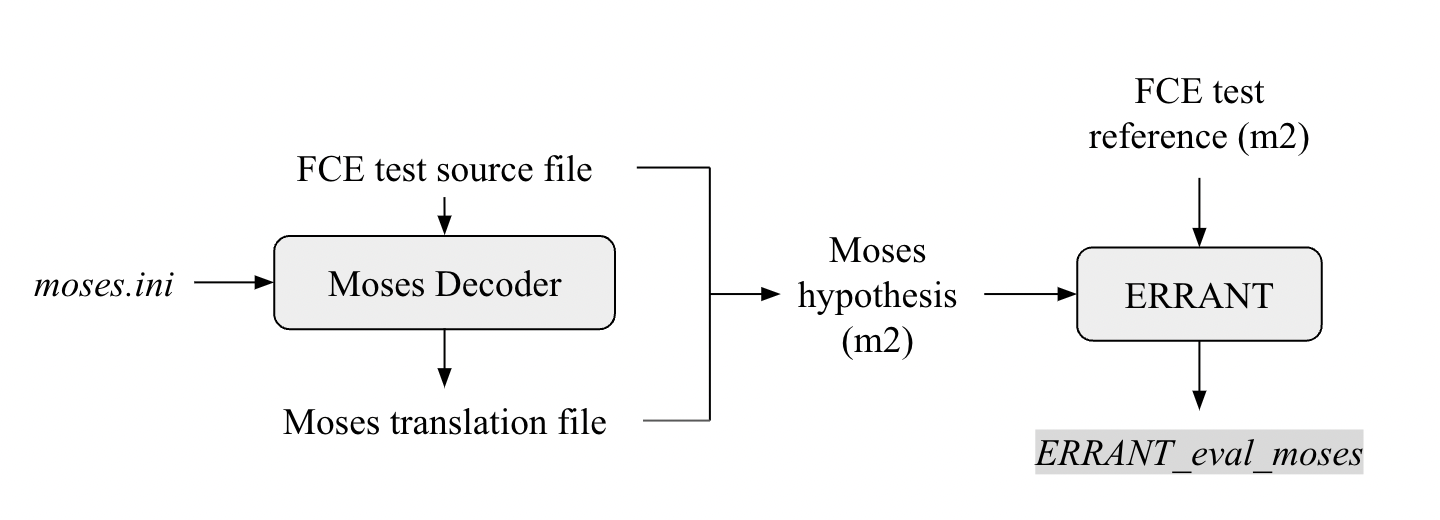
\includegraphics[width=0.9\textwidth]{images/moses_test.png}
\caption{Testing pipeline of the Moses SMT}
\label{fig:moses_test}
\end{figure}

Before testing the Moses decoder, we should tune the parameters using a small amount of parallel data which is different from the training data. The FCE development set was used for this purpose. The tuning process would optimize the weights for each feature as specified in \texttt{moses.ini}. Then we used Moses decoder to translate the test set and produce a hypothesis file which contains the translation given by Moses. The evaluation results were stored in a file named \texttt{ERRANT\_eval\_moses}.


\subsection{\texorpdfstring{R\textsuperscript{2}NN}{R2NN} Decoder}\label{section:r2nn_test}
\begin{figure}[ht]
\centering
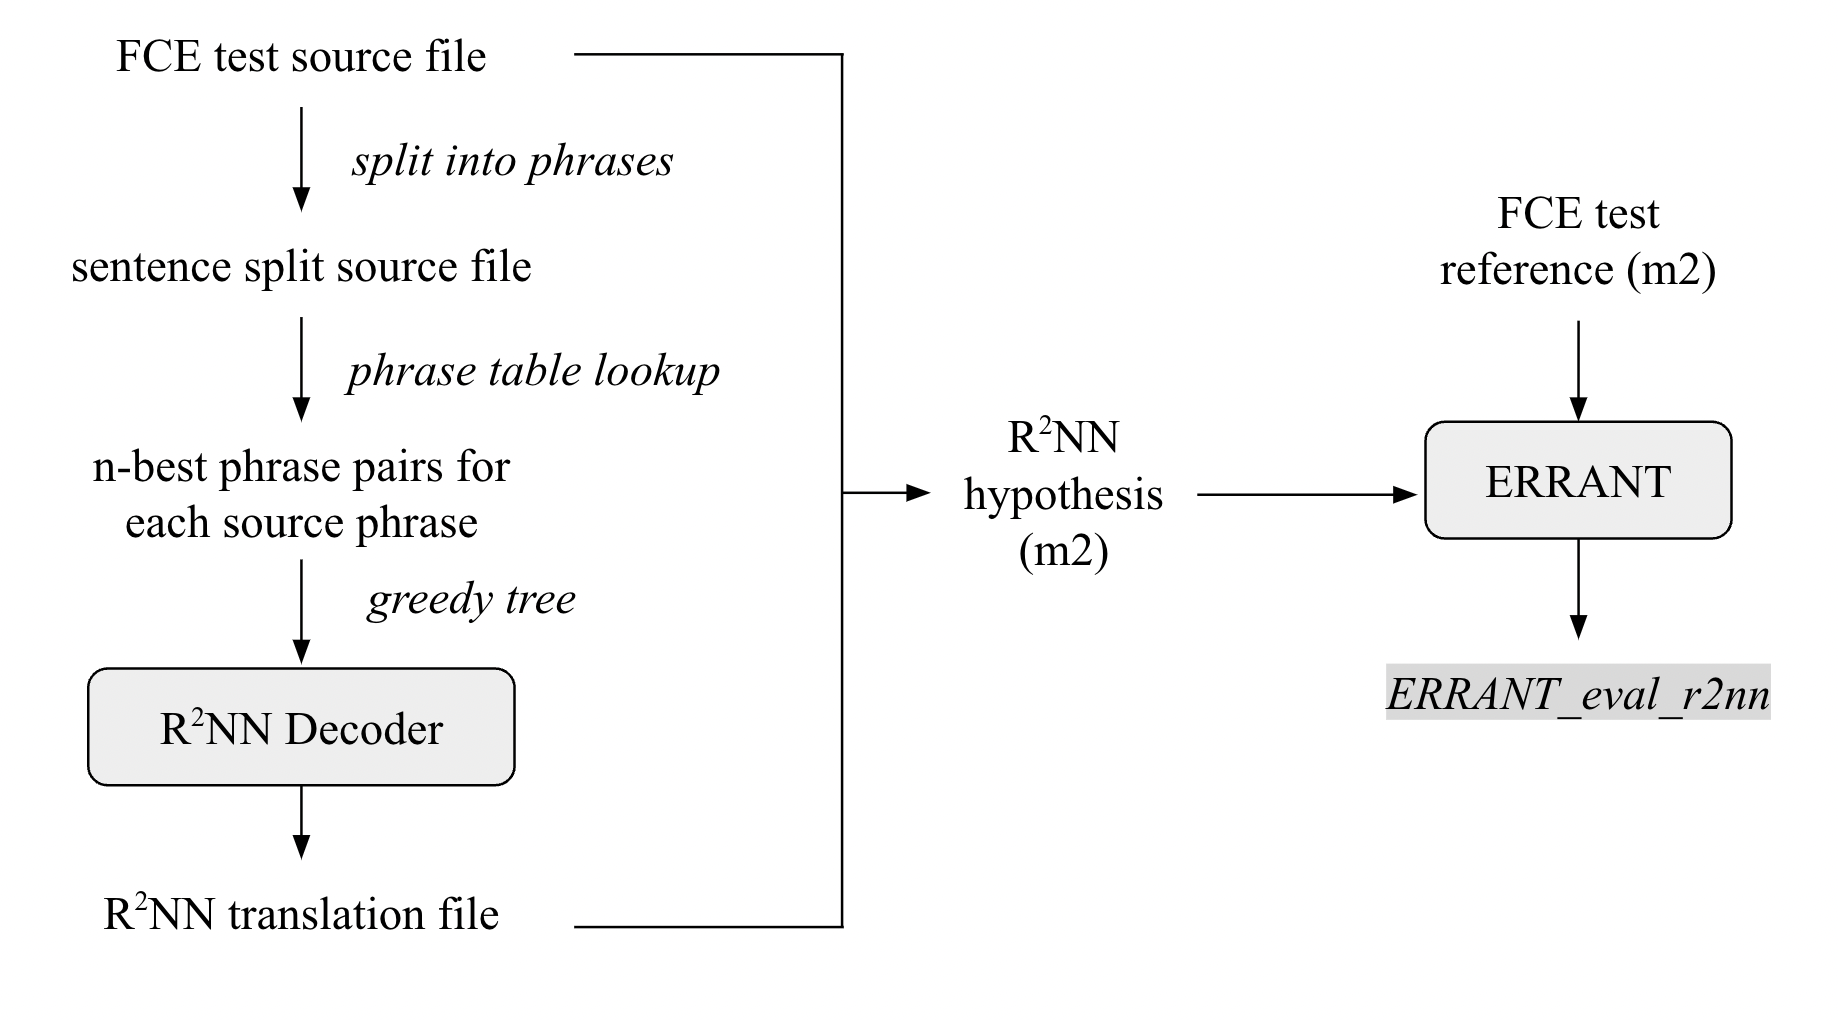
\includegraphics[width=0.8\textwidth]{images/r2nn_test.png}
\caption{Testing pipeline of the R\textsuperscript{2}NN SMT}
\label{fig:r2nn_test}
\end{figure}

To use the R\textsuperscript{2}NN decoder, firstly we need to split the sentence into phrases. Liu et al. did not specify the method they used for phrase splitting in the paper\cite{r2nn}, so I came up with a greedy method: starting from the beginning word of a sentence, we look for the longest possible phrase that appears in our top phrase table. If a phrase is found, we keep the phrase and move on to the remaining part of the sentence; if no such phrases are found, we make that word a phrase, and move on to the next word. An example is given below.

\textbf{Sentence}\\
\textit{I hope that he will recover soon and that he will make it to our conference .}

\textbf{Sentence split}\\
\textit{I hope that / he will / recover / soon and / that he / will make / it to / our / conference / .}

The next step was to obtain phrase pairs based on the sentence split. For each source phrase in the split, we look up the phrase table to obtain a list of possible phrase pairs. The R\textsuperscript{2}NN model was used to compute a score for each phrase pair and only the n-best phrase pairs that gave high scores were kept. Then we recursively repeated the process and built a tree based on the phrase pairs. Every tree node has two attributes: \texttt{node.source} which gives the source phrase of this node and \texttt{node.target} which gives the target phrase. The translation for a sentence can be obtained by accessing the root node's \texttt{target} attribute.

\textbf{Phrase pairs}\\
\textit{(I hope that $\rightarrow$ I hope that),
        (I hope that $\rightarrow$ I hope),
        \dots}

However, when it came to testing, I discovered that the search space was too big for my laptop to process. To process a sentence with $k$ phrases while keeping $n$ best phrase pairs, the number of possible different trees is at least $n^k$. In order to finish testing within a reasonable amount of time, I decided not to keep the n-best phrase pairs but to keep the phrase pair that gives the highest score. The evaluation results of the translation file were saved to \texttt{ERRANT\_eval\_r2nn}.

\section{Results and Discussion}\label{section:results}
Table \ref{table:eval_moses} and \ref{table:eval_r2nn} shows the scores reported by ERRANT for the baseline Moses system and R\textsuperscript{2}NN system.

\begin{table}[ht]
    \centering
    \begin{tabular}{ |c|c|c|c|c|c| } 
     \hline
     TP & FP & FN & Prec & Rec & F0.5 \\ [0.5ex] 
     \hline
     479 & 632 & 4070 & 0.4311 & 0.1053 & 0.2663 \\ 
     \hline
    \end{tabular}
    \caption{ERRANT scorer output for Moses on FCE test set}
    \label{table:eval_moses}
    
    \vspace{1em}
    
    \begin{tabular}{ |c|c|c|c|c|c| } 
     \hline
     TP & FP & FN & Prec & Rec & F0.5 \\ [0.5ex] 
     \hline
     605 & 7088 & 3944 & 0.0786 & 0.133 & 0.0856 \\ 
     \hline
    \end{tabular}
    \caption{ERRANT scorer output for R\textsuperscript{2}NN on FCE test set}
    \label{table:eval_r2nn}
\end{table}

We observe that the $F_{0.5}$ score of R\textsuperscript{2}NN is much lower than the baseline Moses system. Even though R\textsuperscript{2}NN gives a higher recall (lower proportion of missed edits), its precision is lower than that of Moses. Since $F_{0.5}$ weighs precision twice as much as recall, the resulting figure is low. We also observe that R\textsuperscript{2}NN gives more true positive but at the same time much more false positive (FP) than the baseline Moses. It suggests that R\textsuperscript{2}NN tend to make changes to the source sentence even when it should not have. 

Consider the source sentence
\begin{center}
    \textit{Hope you like it .}
\end{center}
The gold reference, as well as the Moses hypothesis, did not make changes to this sentence. On the other hand, the R\textsuperscript{2}NN hypothesis was
\begin{center}
\textit{I hope you like it .}
\end{center}
This contributed to the false negative of the R\textsuperscript{2}NN model. Even though the edit did not change the correctness of the source sentence, it was unnecessary. This edit was made because the source sentence was split into the following phrases
\begin{center}
\textit{Hope you / like it .}
\end{center}
and the best phrase pairs that give the highest score for the R\textsuperscript{2}NN model are
\begin{center}
\textit{Hope you} $\rightarrow$ \textit{I hope you}\\
\textit{like it .} $\rightarrow$ \textit{like it .}
\end{center}

There are two ways to mitigate this problem.
\begin{itemize}
    \item Recall in section \ref{section:r2nn_test}, we only kept the best phrase pair that gives highest score for memory issues. (\textit{Hope you} $\rightarrow$ \textit{I hope you}) was selected because it gave the highest score. Other phrase pairs, including (\textit{Hope you} $\rightarrow$ \textit{Hope you}), were not considered by R\textsuperscript{2}NN for upper tree combination. If we extend it to n-best phrase pairs at the cost of expanding the search space, we would take the correct phrase pair into consideration.
    \item Another possibility is to use a different method to split the source sentence into phrases. For example, if the sentence was split into one phrase (with the phrase being the whole sentence), the correct phrase pair (\textit{Hope you like it .} $\rightarrow$ \textit{Hope you like it .}) would be obtained.
\end{itemize}

The FCE test set also contains sentences with more than one error. Consider the following example:

\textbf{Source sentence}\\
\textit{The best way is definetely , by air .}

\textbf{Gold reference}\\
\textit{The best way is definitely by air .}

\textbf{Moses hypothesis}\\
\textit{The best way is definitely , by air . }

\textbf{R\textsuperscript{2}NN hypothesis}\\
\textit{The best way is definitely by air .}

The source sentence contains multiple orthographic errors: a spelling mistake in \textit{definetely}, and a punctuation mistake in the use of comma. Moses corrected the misspelled word but failed to see the punctuation mistake, whereas the R\textsuperscript{2}NN model captured and corrected both errors successfully.

There are some interesting translation results produced by the R\textsuperscript{2}NN SMT. In the following example, two commas are put next to each other in the source sentence and the quotation mark does not come in pairs.

\begin{center}
    \textit{The most important building of Biasco is the , , Casa Cavalier Pellanda " .}
\end{center}

Both the gold reference and the Moses hypothesis are identical to the source sentence. However, the R\textsuperscript{2}NN model removed the two commas and added an opening quotation mark to match with the closing quotation mark. The R\textsuperscript{2}NN model also removed the word \textit{the} and the ending full stop. 

\textbf{R\textsuperscript{2}NN hypothesis}\\
\textit{The most important building of Biasco is `` Casa Cavalier Pellanda "}

In my opinion, the correct sentence should be
\begin{center}
    \textit{The most important building of Biasco is the `` Casa Cavalier Pellanda " .}
\end{center}
which is different to the gold reference in the dataset. This reflects the complexity of GEC: human annotators do not always agree. It is also interesting that the R\textsuperscript{2}NN captured the punctuation errors of commas and quotation marks, but at the same time introduced more errors by removing the full stop and the article \textit{the}. 

Overall, the R\textsuperscript{2}NN model has its potential: we saw that it successfully spotted some of the errors that were missed by the Moses SMT and even the human annotator. However, it tends to make changes to the original sentences even when the changes are not necessary, resulting in a much higher false positive than Moses. This has two implications: a lower precision as precision measures the proportion of \textbf{correct} edits out of all edits (large denominator), and a higher recall as recall measures the proportion of \textbf{missed} edits. The $F_{0.5}$ score of the R\textsuperscript{2}NN model was lower than the Moses SMT, but future researchers can refer to the implementation of such an R\textsuperscript{2}NN model and more work can be done to improve it.

\chapter{Conclusion}

\section{Summary of Work Completed}
This project fulfilled all of the success criteria as demonstrated in section \ref{section:success_criteria}. In this project, I successfully implemented two SMT-based GEC systems: a phrase-based baseline Moses SMT, and an R\textsuperscript{2}NN SMT. For Moses SMT, I started with building a working SMT system and trained it with FCE data. For R\textsuperscript{2}NN SMT, I constructed phrase pair embedding (TCBPPE) using two neural networks, a feedforward neural network (FNN) and a recurrent neural network (RNN). I implemented the R\textsuperscript{2}NN model from scratch. Then I built the R\textsuperscript{2}NN SMT by integrating TCBPPE and global features such as language model scores into the R\textsuperscript{2}NN decoder. Finally, a comparison was performed on the performance of Moses SMT-based GEC and R\textsuperscript{2}NN SMT-based GEC. R\textsuperscript{2}NN achieved better recall but due to its low precision, overall it gives lower $F_{0.5}$ score than Moses. 

\section{Personal Reflections}
Throughout this project, I gained more insight into neural networks and natural language processing, particularly in the area of grammatical error correction. I learnt how to build a neural network from scratch using PyTorch, and my experience with PyTorch library would certainly be helpful in my future career. 

One important lesson I took from this project is that there will always be unforeseen difficulty. For example, there were some system compatibility problems when I was installing Moses. There were times when my system would complain about running low on memory and stopped execution before it could produce any meaningful data after running for hours. There is no way I could predict all that, but the best I could do is to allow extra time for each task and do not leave it until the last minute. Another fact that I did not realise is that it is challenging to build a neural network from scratch, especially when the neural network has a novel structure. If I was going to start this project again, I would have put more time into constructing the recursive recurrent neural network (R\textsuperscript{2}NN) because it was far more challenging than the theory in the paper\cite{r2nn} looked like.

\section{Future Work}
Due to the time constraint of this project, I did not refine the R\textsuperscript{2}NN SMT further but there are several possible ways to improve its performance.

\begin{enumerate}
    \item Inevitably, unseen word will exist no matter how big our training set is, especially for the task of GEC where the input data could contain misspelled words. In my implementation of the R\textsuperscript{2}NN, I kept the original word/phrase for unseen data. This may ignore errors like spelling mistakes. Alternatively we could expand the size of phrase tables at the cost of memory and searching time.
    
    \item Recall in section \ref{section:r2nn_test}, I only kept the best phrase pair for upper tree combination to avoid having a huge search space. It is more sensible to keep n-best phrase pairs so that our model can consider the possibility of a tree which does not use all of \textit{the best} phrase pairs and yet produce a higher score.
    
    \item The dataset used to train our R\textsuperscript{2}NN SMT system is small. We could use other training data available on BEA 2019\cite{bryant-etal-2019-bea} in addition to the FCE dataset.
    
    \item Before a sentence is passed to the R\textsuperscript{2}NN, it has to be split into phrases. The way I split the sentence is described in section \ref{section:r2nn_test}, but other algorithms to split the sentence may be used to obtain different initial phrases and hence different initial tree leaves.
\end{enumerate}


%%%%%%%%%%%%%%%%%%%%%%%%%%%%%%%%%%%%%%%%%%%%%%%%%%%%%%%%%%%%%%%%%%%%%
% the bibliography
\addcontentsline{toc}{chapter}{Bibliography}
\bibliography{refs}

%%%%%%%%%%%%%%%%%%%%%%%%%%%%%%%%%%%%%%%%%%%%%%%%%%%%%%%%%%%%%%%%%%%%%
% the appendices
\appendix

\chapter{Code Implementation}

\section{TreeNode}
\begin{lstlisting}
class TreeNode:
    def __init__(self, vector=None, source="", target=""):
        self.vector = vector
        self.source = source
        self.target = target
        self.left = None
        self.right = None

    def greedy_tree(self, sentence_span_tuple, model):
        sentence_span = [[tup[0] for tup in pair] for pair in sentence_span_tuple]
        num_pairs = len(sentence_span)
        leafs = []
        for pair_id in range(num_pairs):
            source_phrase = sentence_span[pair_id][0]
            target_phrase = sentence_span[pair_id][1]
            pair_rec = get_rec(source_phrase, target_phrase)
            pair_ppe = get_ppe(source_phrase, target_phrase)
            pair_vector = torch.concat((pair_rec, pair_ppe), 0)

            leaf_node = TreeNode(vector=pair_vector, source=source_phrase, target=target_phrase)
            leafs.append(leaf_node)

        while len(leafs) >= 2:
            max_score = float('-inf')
            max_hypothesis = None
            max_idx = None
            for i in range(1, len(leafs)):
                hypothesis = TreeNode()
                hypothesis.left = leafs[i - 1]
                hypothesis.right = leafs[i]
                vector, score = model(hypothesis)
                hypothesis.vector = vector
                hypothesis.source = hypothesis.left.source + " " + hypothesis.right.source
                hypothesis.target = hypothesis.left.target + " " + hypothesis.right.target
                if score > max_score:
                    max_score = score
                    max_hypothesis = hypothesis
                    max_idx = i
            leafs[max_idx - 1:max_idx + 1] = [max_hypothesis]
        return leafs[0]
\end{lstlisting}

\section{\texorpdfstring{R\textsuperscript{2}NN}{R2NN}}
\begin{lstlisting}
class R2NN(torch.nn.Module):
    def __init__(self, ppe_size, rec_size):
        super(R2NN, self).__init__()
        self.input_size = ppe_size + rec_size
        self.W = torch.nn.Linear(self.input_size * 2, ppe_size, dtype=torch.float32)
        self.V = torch.nn.Linear(self.input_size, 1, dtype=torch.float32)

    def forward(self, node):
        left_node_vector = torch.zeros([self.input_size], dtype=torch.float32)
        left_node_source = ""
        left_node_target = ""
        right_node_vector = torch.zeros([self.input_size], dtype=torch.float32)
        right_node_source = ""
        right_node_target = ""

        if node.left is None and node.right is None:
            left_node_vector = node.vector
            left_node_source = node.source
            left_node_target = node.target
        if node.left is not None:
            left_node_vector = node.left.vector
            left_node_source = node.left.source
            left_node_target = node.left.target
        if node.right is not None:
            right_node_vector = node.right.vector
            right_node_source = node.right.source
            right_node_target = node.right.target

        inp_vector = torch.cat([left_node_vector, right_node_vector], 0)
        parent_ppe = torch.tanh(self.W(inp_vector))

        parent_source = left_node_source + " " + right_node_source
        parent_target = left_node_target + " " + right_node_target
        parent_rec = get_rec(parent_source, parent_target)

        parent = torch.cat([parent_rec, parent_ppe], 0)
        output = self.V(parent)
        return parent, output
\end{lstlisting}


\chapter{Project Proposal}
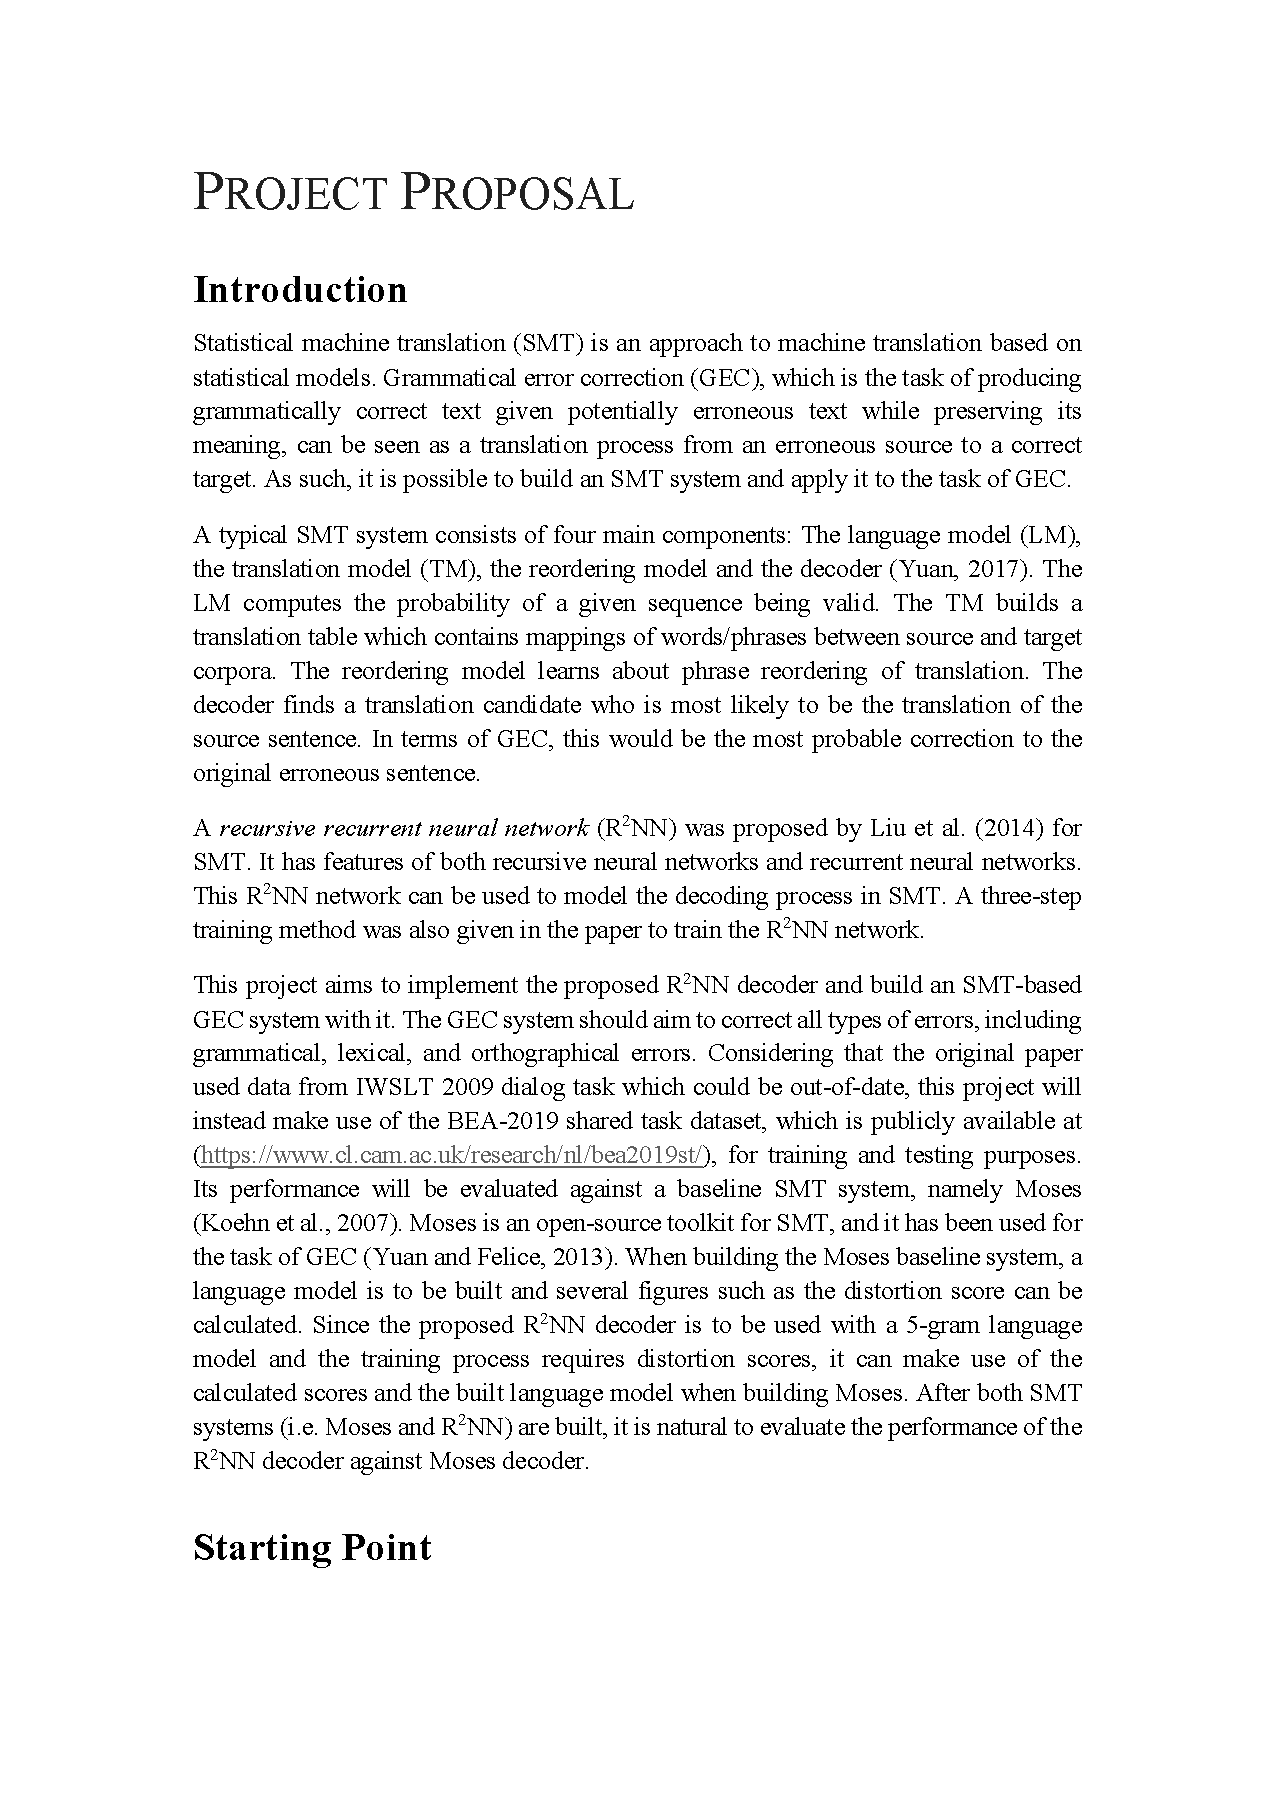
\includepdf[pages=-]{proposal.pdf}

\end{document}